\documentclass[]{book}
\usepackage{lmodern}
\usepackage{amssymb,amsmath}
\usepackage{ifxetex,ifluatex}
\usepackage{fixltx2e} % provides \textsubscript
\ifnum 0\ifxetex 1\fi\ifluatex 1\fi=0 % if pdftex
  \usepackage[T1]{fontenc}
  \usepackage[utf8]{inputenc}
\else % if luatex or xelatex
  \ifxetex
    \usepackage{mathspec}
  \else
    \usepackage{fontspec}
  \fi
  \defaultfontfeatures{Ligatures=TeX,Scale=MatchLowercase}
\fi
% use upquote if available, for straight quotes in verbatim environments
\IfFileExists{upquote.sty}{\usepackage{upquote}}{}
% use microtype if available
\IfFileExists{microtype.sty}{%
\usepackage{microtype}
\UseMicrotypeSet[protrusion]{basicmath} % disable protrusion for tt fonts
}{}
\usepackage[margin=1in]{geometry}
\usepackage{hyperref}
\hypersetup{unicode=true,
            pdftitle={Text Mining Techniques for Knowledge Extraction from Technical Documents},
            pdfauthor={Filippo Chiarello},
            pdfborder={0 0 0},
            breaklinks=true}
\urlstyle{same}  % don't use monospace font for urls
\usepackage{natbib}
\bibliographystyle{apalike}
\usepackage{longtable,booktabs}
\usepackage{graphicx,grffile}
\makeatletter
\def\maxwidth{\ifdim\Gin@nat@width>\linewidth\linewidth\else\Gin@nat@width\fi}
\def\maxheight{\ifdim\Gin@nat@height>\textheight\textheight\else\Gin@nat@height\fi}
\makeatother
% Scale images if necessary, so that they will not overflow the page
% margins by default, and it is still possible to overwrite the defaults
% using explicit options in \includegraphics[width, height, ...]{}
\setkeys{Gin}{width=\maxwidth,height=\maxheight,keepaspectratio}
\IfFileExists{parskip.sty}{%
\usepackage{parskip}
}{% else
\setlength{\parindent}{0pt}
\setlength{\parskip}{6pt plus 2pt minus 1pt}
}
\setlength{\emergencystretch}{3em}  % prevent overfull lines
\providecommand{\tightlist}{%
  \setlength{\itemsep}{0pt}\setlength{\parskip}{0pt}}
\setcounter{secnumdepth}{5}
% Redefines (sub)paragraphs to behave more like sections
\ifx\paragraph\undefined\else
\let\oldparagraph\paragraph
\renewcommand{\paragraph}[1]{\oldparagraph{#1}\mbox{}}
\fi
\ifx\subparagraph\undefined\else
\let\oldsubparagraph\subparagraph
\renewcommand{\subparagraph}[1]{\oldsubparagraph{#1}\mbox{}}
\fi

%%% Use protect on footnotes to avoid problems with footnotes in titles
\let\rmarkdownfootnote\footnote%
\def\footnote{\protect\rmarkdownfootnote}

%%% Change title format to be more compact
\usepackage{titling}

% Create subtitle command for use in maketitle
\newcommand{\subtitle}[1]{
  \posttitle{
    \begin{center}\large#1\end{center}
    }
}

\setlength{\droptitle}{-2em}

  \title{Text Mining Techniques for Knowledge Extraction from Technical Documents}
    \pretitle{\vspace{\droptitle}\centering\huge}
  \posttitle{\par}
    \author{Filippo Chiarello}
    \preauthor{\centering\large\emph}
  \postauthor{\par}
      \predate{\centering\large\emph}
  \postdate{\par}
    \date{2018-09-24}

\usepackage{booktabs}

\begin{document}
\maketitle

{
\setcounter{tocdepth}{1}
\tableofcontents
}
\chapter{Introduction}\label{introduction}

\section{Goal}\label{goal}

Il problema non è sostituire domain knowledge. Idea vecchia ha fallito.
E' insostibuibile perchè:

\begin{itemize}
\tightlist
\item
  Technology, interessa gli ingegneri
\item
  Social Science, decision making
\end{itemize}

PErchè fallita: da una parte è andata avanti la knowledge
rappresentation. E' impossibile rappresentare la conoscenza con regole,
ma con altri strumenti si può rappresentare (bottom-up).

Inoltre ho text mining, capaità di processare testi. Parte di
intelligenza artificiale. Questi fenomeni non sostituioscono l'esperto
ma ne cambiano il modo di operare.

Oggi si integra. Vogliamo un esperto di dominio che faccia meglio il suo
mestiere.

Abbiamo oggi più potenza e correzione errori.

Oltre ad efficienza e potenza nel correggere gli errori. Ora c'è anche
la possibilità dio maggiore specificità. L'obiettivo è qiuindi poratre
domain knowledge sia su technology sia ai decisori sociali.

\section{Problem}\label{problem}

Foresight

\section{Solutions}\label{solutions}

\begin{figure}

{\centering 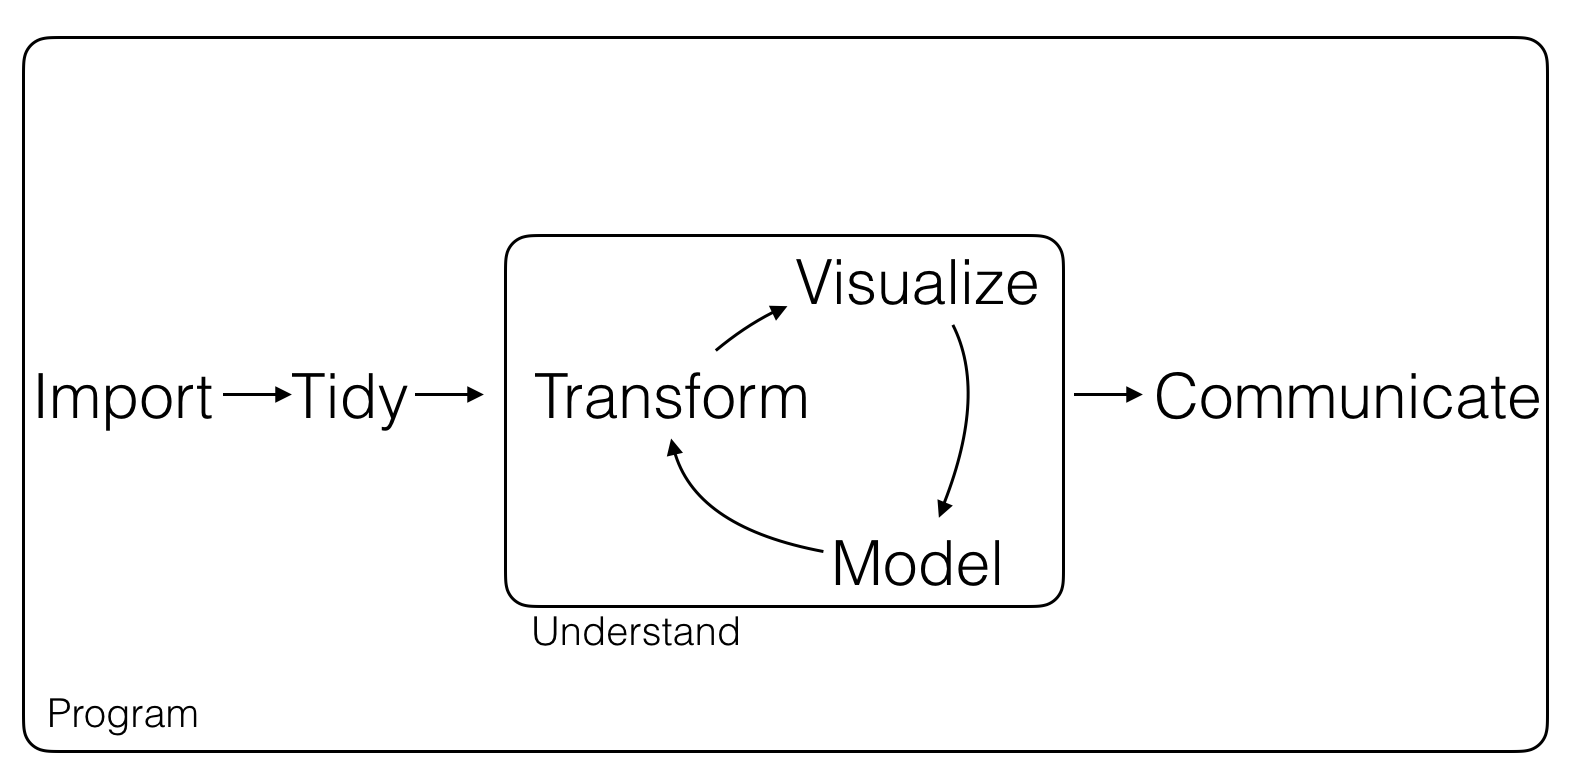
\includegraphics[width=0.8\linewidth]{_bookdown_files/figures/main_work_flow} 

}

\caption{A general workflow for the process of data analysis. Readapted from Wickham (2016)}\label{fig:mainworkflow}
\end{figure}

\section{Challenges: Understanding and
Programming}\label{challenges-understanding-and-programming}

\subsection{Understanding}\label{understanding}

\subsection{Programming}\label{programming}

\section{Research Questions}\label{research-questions}

\section{Stakeholders}\label{stakeholders}

Marketing

Research and Development

Design

Human Resources

Other Stakeholders

\section{Knowledge Intensive Manegement
Engineering}\label{knowledge-intensive-manegement-engineering}

Tipicamente occupaimo di attività ad altà ripetitività. Ti porti dietro
metodologie ingegneristiche applicate a sistemi inernti, andnano a
operare in sistemi socio-tecnici. Hai fatto il tuo mestieri (ricerca
operativa ecc..). Negli ultimi anni però le aziende le attività a
maggior valore aggiunto sono non ripetitive. R\&S, Design, marketing, HR
ecc.. e quindi gestione della conoscena. Su situazione che sembrano
uniche il gestionale rischia di perdere rispetto al creativo. Come
disciplina voglio presidiare queste aree: non ci occupaimo di casi
unici, ma costruire modelli in grado di incorporare conoscenza per
essere usati in questi. La tesi ha l'obbiettivo di esploration and
exploitation queste direzioni. Hon trovato nella data science è più
nello specifico nel text mining gli strumenti adatti.

\chapter{State of the Art}\label{sota}

The analysis of technical documents require the design of processes that
rely both on programming and Natural Language Processing techniques and
on the understanding and knowledge of field experts. While the first
techniques are codified and explicit, the second are sometimes implicit
and always harder to systematize. In this section i treat these two
groups of techniques in the same way to give to the reader a systematic
literature review on these topics. For this reason the sections of this
chapter has the subsequent structure:

\begin{itemize}
\tightlist
\item
  At a first level there are two sections \ref{sotatools} and
  \ref{sotadocuments}, reviewing respectively the processes of
  \emph{programming and Natural Language Processing} and of
  \emph{undestanding and knowldege of field experts application};
\item
  Section \ref{sotatools} has a subsection for each of the \emph{phases}
  showed in figure \ref{fig:mainworkflow}. These subsections goes from
  \ref{sotatoolsprogram} to \ref{sotatoolscomunicate};
\item
  Each subsection from \ref{sotatoolsprogram} to
  \ref{sotatoolscomunicate} contains the relative Natural Language
  Processing \emph{task} that are relevant for the analysis of technical
  documents, for example Document Retrieval
  \ref{sotatoolsimportretrieval}, Part-Of-Speech-Tagging;
  \ref{sotatoolstransformpos} or Named Entity Recognition
  \ref{sotatoolsmodelner}.
\item
  Each task subsection describes the relevant \emph{techniques} to
  perform that task. I use the word techniques to include mainly
  algorithms and procedures but also more generic methods or frameworks;
\item
  Since the second section \ref{sotadocuments} describes less systematic
  phases, task and techniques this section opens with a first subsection
  \ref{sotadocumentsunderstand} that focuses on the studies of the
  problems of using expert knowledge in an analytic process and which
  are the techniques to convert this knowledge in a format that is
  usable in a Natural Language Processing workflow.
\item
  Finally, always section \ref{sotadocuments} has a subsection for each
  of the anlyzed technical \emph{documents}. These subsections goes from
  \ref{sotadocumentspatents} to \ref{sotadocumentsjobs}.
\end{itemize}

\section{Phases, Tasks, and Techniques}\label{sotatools}

In this section I make a review of the most important techniques for
Natural Language Processing in the context of technical documents
analysis. The techniques (mainly algorithms) are grouped in phases
(Import, Tidy, Transform, Model, Visualize, Communicate) showed in
figure \ref{fig:mainworkflow} and each phases is dived in the NLP tasks
that are the most important for the analysis of technical documents.
This standard process has been disclosed in the framework of the
tidyverse \citep{wickham2016r}. The algorithms i reviewed in this
section are summmarised in table tot, where the reader can see the
relationship between tasks and techniques.

\subsection{Program}\label{sotatoolsprogram}

Programming is a key activity to perform in order to effectively and
efficiently perform text mining. It is not a phases per se because each
phase is implemented trough programming. It is critical that an analysts
has in mind the need of maximizing the probability that their analysis
is reproducible, accurate, and collaborative. This goals can be reached
only trough programming. The most used programming languages for text
mining and natural language processing are R \citep{r2008} and Python
\citep{py95}. R and Python are both open-source programming languages
with a large community of developers, and new libraries or tools are
added continuously to their respective catalog. R is mainly used for
statistical analysis and data science while Python is a more general
purpose programming language. R has been developed by Academics and
statisticians over two decades. R has now one of the richest ecosystems
to perform data analysis and there are around 12000 packages available
in CRAN (open-source repository of R). The rich variety of libraries
makes R the first choice for statistical analysis. Another cutting-edge
difference between R and the other statistical products is R-studio.
RStudio is a free and open-source integrated development environment
(IDE) for R. It includes a console, syntax-highlighting editor that
supports direct code execution, as well as tools for plotting, history,
debugging and workspace management. Finally, it is widely recognized the
great performances that R has for data visualisation and communication.
Python can pretty much do the same tasks as R: data wrangling,
engineering, feature selection web scrapping, app and so on. Anyway,
Python has great performances in the deployment and implementation of
machine learning at a large-scale. Furthermore, Python codes are easier
to maintain and more robust than R.

\subsection{Import}\label{sotatoolsimport}

The first activities to perform in a text mining pipeline is to find all
the documents that contains useful information for the analysis and then
import the corpus (the set of documents) in to the computer program. The
present section is thus focused on techniques for document retrieval
\ref{sotatoolsimportretrieval} and on the most popular documents digital
formats \ref{sotatoolsimportformat}.

\subsubsection{Document Retrieval}\label{sotatoolsimportretrieval}

Document retrieval is the process of matching a user query against a set
of documents. A document retrieval system has two main tasks:

1- Find the documents that are relevant with respect to the user queries
2- Measure the relevance of the matching results

Building a query means to use field specific knowledge and logical rules
to write a text string that is the composition of keywords and Boolean
operators. The set of keywords (single words or phrases) is chosen in
such a way that these are likely to be contained in the searched
documents. Boolean operators can also be used to increment the
performance of the query. The AND operator, for example is used to
retrieve all the document that contains both of the terms at the left
and the right of it, OR for document that contains at least one of the
two words. Another important tool for making a good query are regular
expressions. Regular expression (regexp) is a language for specifying
text search strings, an algebraic notation for characterizing a set of
strings. This language widely used in modern word processor and text
processing tools. A regular expression search function will search
through the corpus, returning all texts that match the pattern. For
example, the Unix command-line tool grep takes a regular expression and
returns every line of the input document that matches the expression. To
evaluate the performance of a query is useful to understand the concepts
of precision and recall.

Recall is the ratio of relevant results returned to all relevant
results. Precision is the number of relevant results returned to the
total number of results returned. Due to the ambiguities of natural
language, full-text-search systems typically includes options like stop
words to increase precision. Stop-words are words that filter all the
document which contains them. On the other side, stemming to increase
recall \ref{sotatoolstransformstemming}. The trade-off between precision
and recall is simple: an increase in precision can lower overall recall,
while an increase in recall lowers precision \citep{yuwono1996search}.
Usually when a user performs a query, the main problem are false
positives (the results that are returned by the systems but are not
relevant to the user). False positives has a negative impact on the
precision of the query. The retrieval of irrelevant documents is
particularly strong for technical documents due to the inherent
ambiguity of technical language. For this reason to understand and to
use the rules of query building are fundamental to the technical
document analysis, since without a good query is rare to have a good set
of documents to analyze.

\subsubsection{Documents Format}\label{sotatoolsimportformat}

For the purpose of the present thesis documents are considered in a
digital format, and there is no need to read it from a analogical
source. From the computer science point of view, text is a
human-readable sequence of characters and the words they form that can
be encoded into computer-readable formats. There is no standard
definition of a text file, though there are several common formats. The
most common types of encoding are:

\begin{itemize}
\tightlist
\item
  ASCII, UTF-8 --- plain text formats
\item
  .doc for Microsoft Word --- Structural binary format developed by
  Microsoft (specifications available since 2008 under the Open
  Specification Promise)
\item
  HTML (.html, .htm), (open standard, ISO from 2000)
\item
  Office Open XML --- .docx (XML-based standard for office documents)
\item
  OpenDocument --- .odt (XML-based standard for office documents)
\item
  PDF --- Open standard for document exchange. ISO standards include
  PDF/X (eXchange), PDF/A (Archive), PDF/E (Engineering), ISO 32000
  (PDF), PDF/UA (Accessibility) and PDF/VT (Variable data and
  transactional printing). PDF is readable on almost every platform with
  free or open source readers. Open source PDF creators are also
  available.
\item
  Scalable Vector Graphics (SVG) - Graphics format primarily for
  vector-based images.
\item
  TeX --- Popular open-source typesetting program and format. First
  successful mathematical notation language.
\end{itemize}

For the R software there exist many packages that helps to import
documents in several formats \citep{readr2017r}.

\subsection{Tidy}\label{sotatoolstidy}

After that data are imported they have to be processed in such a way
that it would be possible to perform the main task of data analysis
(transformation, modelling and visualisation). This task of tidying data
(usually referred to as data pre-processing) can be very time expensive,
so it is important to have clear methods and techniques to perform this
task.

Tidy data sets have structure and working with them is easy; they're
easy to manipulate, model and visualize \citep{wickham2014tidy}. Tidy
data sets main concept is to arrange data in a way that each variable is
a column and each observation (or case) is a row. The characteristics of
tidy data can be thus summarised as the points \citep{leek2015elements}:

\begin{itemize}
\tightlist
\item
  Each variable you measure should be in one column
\item
  Each different observation of that variable should be in a different
  row
\item
  If you have multiple tables, they should include a column in the table
  that allows them to be linked
\end{itemize}

There main advantages of structuring the data in this way is that a
consistent data structure make it easier to use the tools (programs)
that work with it because they have an underlying uniformity. This lead
to an advantage in reproducibility of code.

As stated before tidying data is not a trivial task, and applying this
process to text is even harder for documents with respect to structured
data \citep{silge2016tidytext}. On the other side, is clear that using
tidy data principles can make many text mining tasks easier, more
effective, and consistent with tools already in wide use . Treating text
as data frames of individual words allows us to manipulate, summarize,
and visualize the characteristics of text easily and integrate natural
language processing into effective workflows already used.

Tidy text format is designed as being a table with one-token-per-row. A
token unit of text that is meaningful for the analysis to be performed
(for example letters, words, n-gram, sentences, or paragraphs ).
Tokenization is the process of splitting text into tokens. This
one-token-per-row structure is in different from the ways documents are
often stored in current analyses, mainly strings or document-term
matrix. The term document matrix has each corpus word represented as a
row with documents as columns. The document term matrix is the
transposition of the TDM so each document is a row and each word is a
column. The term document matrix or document term matrix is the
foundation of bag of words text mining. The bag-of-words model is a
simplifying representation of documents: a text is represented as the
bag (multiset) of its words, disregarding grammar and even word order
but keeping multiplicity \citep{mctear2016conversational}.

\subsection{Transform}\label{sotatoolstransform}

Transforming in the context of Natural Language Processing is what in
computational linguistic is called text normalization. Normalizing text
means converting it to a more convenient, standard form. Most of the
task of technical document analysis in fact relies on first separating
out or tokenizing sentences and words, strip suffixes from the end of
the word, determining the root of a word or transform the text using
regular expressions.

\subsubsection{Sentence Splitting}\label{sentence-splitting}

The analysis of technical documents require as first process, that the
input text is segmented in sentences. Since documents do not encode this
information in a non ambiguous manner (using dots) due to common
abbreviations (e.g.: ``Mr., Dr.''), a sentence splitting process that
does not rely only on a trivial \emph{dot based} rule is required. This
issue in the technical documents domain is even more problematic due to
the presence of formulas, numbers, chemical entity names and
bibliographic references. Furthermore, since sentence splitting is one
of the first processes of an NLP pipeline, errors in this early stage
are propagated in the following steps causing a strong decrease for what
concerns their accuracy. One of the most advanced techniques are machine
learning techniques: given a training corpus of properly segmented
sentences and a learning algorithm, a statistical model is built. By
reusing the statistical model, the sentence splitter is able to split
sentences on texts not used in the training phase. ItalianNLP lab
systems uses this approach \citep[\citet{attardi2009reverse},
\citet{attardi2009accurate}]{dell2009ensemble}. For this reason this
algorithm is used for the most of the application presented in this
Thesis.

\subsubsection{Tokenization}\label{tokenization}

Since documents are unstructured information, these has to be divided
into linguistic units. The definition of linguistic units is
non-trivial, and more advanced techniques can be used (such as n-gram
extraction) but most of the times these are words, punctuation and
numbers. English words are often separated from each other by white
space, but white space is not always sufficient. Solving this problems
and splitting words in well-defined tokens defined as tokenization. In
most of the application described in the present Thesis, the tokenizer
developed by the ItalianNLP lab was integrated
\citep{dell2009ensemble, attardi2009reverse, attardi2009accurate}. This
tokenizer is regular expression based: each token must match one of the
regular expression defined in a configuration file. Among the others,
rules are defined to tokenize words, acronyms, numbers, dates and
equations.

\subsubsection{Stemming}\label{sotatoolstransformstemming}

Stemming is a simpler but cruder methodology for chopping off of
affixes. The goal of stemming is reducing inflected (or sometimes
derived) words to their word stem, base or root form. The stem of a word
and its morphological root do not need to be identical; it is sufficient
that related words map to the same stem, even if this stem is not a
valid root. One of the most widely used stemming is the simple and
efficient Porter algorithm \citep{porter1980algorithm}.

\subsubsection{Lemmatisation}\label{sotatoolstransformlemmatisation}

Lemmatization is the task of determining the root of a words. The output
allow to find that two words have the same root, despite their surface
differences. For example, the verbs \emph{am}, \emph{are}, and \emph{is}
have the shared lemma \emph{be}; the nouns \emph{cat} and \emph{cats}
both have the lemma \emph{cat}. Representing a word by its lemma is
important for many natural language processing tasks. Lemmatisation in
fact diminish the problem of sparsity of document-word matrix.
Furthermore lemmatisaion is important for document retrieval
\ref{sotatoolsimportretrieval} web search, since the goal is to find
documents mentioning motors if the search is for motor. The most recent
methods for lemmatization involve complete morphological parsing of the
word \citep{hankamer1989morphological}.

\subsubsection{Words importance metrics}\label{sotatoolstransformwi}

Once that a document has been tokenized and the tokens has been
transformed, an analyst usually wants to measure how important a word is
to a document in a collection or corpus. Some of the metrics adopted
are:

\begin{itemize}
\tightlist
\item
  \emph{Term Frequency}: the number of times that a term occurs in
  document.
\item
  \emph{Boolean frequency}: 1 if the term occurs in the document and 0
  otherwise;
\item
  \emph{Term frequency adjusted for document length}: is raw count
  normalized for the number of words contained in the document
\item
  \emph{Logarithmically scaled frequency}: is raw count normalized for
  the natural logarithm of one plus the number of words contained in the
  document
\item
  \emph{Inverse document frequency}: is the logarithmically scaled
  inverse fraction of the documents that contain the word, obtained by
  dividing the total number of documents by the number of documents
  containing the term, and then taking the logarithm of that quotient.
  It is a measure of how much information the word provides, that is,
  whether the term is common or rare across all documents.
\item
  \emph{Term frequency--Inverse document frequency}: the product between
  \emph{term frequency and inverse document frequency}. A high weight in
  tf--idf is reached by a high term frequency (in the given document)
  and a low document frequency of the term in the whole collection of
  documents; the weights hence tend to filter out common terms.
\end{itemize}

\subsubsection{Part-of-Speech Tagging}\label{sotatoolstransformpos}

The part of speech plays an central role in technical document analysis
since it provides very useful information concerning the morphological
role of a word and its morphosyntactic context: for example, if a token
is a determiner, the next token is a noun or an adjective with very high
confidence. Part of speech tags are used for many information extraction
tools such as named entity taggers (see section \ref{sotatoolsmodelner})
in order to identify named entities. In typical named entity task these
are people and locations since tokens representing named entities follow
common morphological patterns (e.g.~they start with a capital letter).
For the application to technical documents, technical entities (like the
possible failures of a manufact) becomes more relevant. In this context
a correct part-of-speech tagger becomes even more important since
morphosyntactical rules can not be used. In addition part of speech tags
can be used to mitigate problems related to polysemy since words often
have different meaning with respect to their part of speech (e.g.
``track'', ``guide''). This information is extremely valuable in patent
analysis, and some patent tailored part-of-speech tagger has been
designed (see section \ref{sotadocumentspatents}). The literature on
pos-tagger is huge, and goes behind the scope of the present thesis to
make a complete review. In most of the application presented in this
work, was employed the ILC postagger \citep{attardi2006experiments}.
This postagger uses a supervised training algorithm: given a set of
features and a training corpus, the classifier creates a statistical
model using the feature statistics extracted from the training corpus.

\subsection{Model}\label{sotatoolsmodel}

The goal of a model is to provide a simple low-dimensional summary of a
dataset \citep{wickham2016r}. Ideally, the model will capture patterns
generated by the phenomenon of interest (true signals), and ignore
random variations (noise). A good model at the same time is able to
capture the weak signals that cab be easily confounded with noise. These
information is particularly valuable in the context of technical
document analysis, where great technical insight could come weak
quasi-invisible signals. \citep{james2013introduction}

Probabilistic models are widely used in text mining nowadays, and
applications range from topic modeling, language modeling, document
classification and clustering to information extraction. The present
section contains a review of the most used methods used to model textual
information.

\subsubsection{N-Grams}\label{sotatoolstransformngrams}

An n-gram is a sequence of N n-gram words: a 2-gram (or bigram) is a
two-word sequence of words like ``credit card'', ``3d printing'', or
''printing machine'', and a 3-gram (or trigram) is a three-word sequence
of words like ``3d printing machine''. Statistical model can be used to
extract the n-grams contained in a document. A first approach has the of
predicting the next item in a sequence in the form of a (n − 1)--order
Markov model\citep{lafferty2001document}. The algorithm begin with the
task of computing P(w\textbar{}h), the probability of a word w given a
word h.The way to estimate this probability is using relative frequency
counts. To do that the algorithms count the number of times h is
followed by the w. With a large enough corpus it is possible to build
valuable models, able to extract n-grams
\citep{bellegarda2004statistical}. While this method of estimating
probabilities directly from counts works for many natural language
applications, in many cases a huge dimension of the corpus does make the
model useful, and this is particularly true for technical documents
\citep{brants2012large}. This is because technical language has a strong
ratio of evolution; as new artifact are invented, new chunks are created
all the time, and has no sense to continuously count every word
co-occurrence to update our model\citep{gibson1994tools}. A more useful
method for chunk extraction fro technical document uses
part-of-speech-tagging and regular expression. Once a document is
pos-taggerd each word is associated whit a particular part of speech:
each sentence is represented as a sequence of part-of-spech. Once this
representation is ready, it is possible to extract only certain
sequences of part-of-speeches, the ones that whit an high level of
confidence are n-grams.

\subsubsection{Document Classification}\label{sotatoolsmodeldocclass}

Classification is a general process that has the goal of taking an
object, extract features, and assign to the observation one of a set of
discrete classes. This process is largely used for documents
\citep{borko1963automatic} and there exist many methods for document
classification \citep{aggarwal2012survey}.

Regardless of technological sector, most organizations today are facing
the problem of overload of information. When it comes to classify huge
amount of documents or to separate the useful documents from the
irrelevant, document classification techniques can reduce the process
cost and time.

The simplest method for classifying text is to use expert defined rules.
These systems are called expert systems or knowledge engineering
approach. Expert rule-based systems are programs that consist of rules
in the IF form condition THEN action (if condition, then action). Given
a series of facts, expert systems, thanks to the rules they are made of,
manage to deduce new facts. The expert systems therefore differ from
other similar programs, since, by referring to technologies developed
according to artificial intelligence, they are always able to exhibit
the logical steps that underlie their decisions: a purpose that, for
example, is not feasible from the human mind or black box-systems. There
are many type of documents for which expert based classifiers constitute
a state-of-the-art system, or at least part of it. Anyway, rules can be
useless in situations such as: - data change over time - the rules are
too many and interrelated

Most systems of documents classification are instead done via supervised
learning: a data set of input observations is available and each
observation is associated with some correct output (training set). The
goal of the algorithm is to build a static model able to learn how to
map from a new observation (test set) to a correct output. The
advantages of this approach over the knowledge engineering approach are
a very good effectiveness, considerable savings in terms of expert labor
power, and straightforward portability to different domains.

In the supervised document classification process, is used a training
set of N documents that have each been typically hand-labeled with a
class: (d1, c1),\ldots{}.,(dN, cN). I say typically, because other less
expensive methods could be designed, as it will be shown for the task of
Named Entity Recognition (another supervised learning task, that
classifies words instead of documents \ref{sotatoolsmodelner}). The goal
of the supervised document classification task is to learn a statistical
model capable of assign a new document d to its correct class c ∈ C.
There exist a class of these classifier, probabilistic classifiers, that
additionally will tell us the probability of the observation being in
the class.

Many kinds of machine learning algorithms are used to build classifiers
\citep{aggarwal2012survey}, such as:

\begin{itemize}
\item
  \emph{Decision Tree Classifiers}: Decision tree documents classifier
  are systems that has as output a classification tree
  \citep{sebastiani2002machine}. In this tree internal nodes are terms
  contained in the corpus under analysis, branches departing are labeled
  by the weight (see section \ref{sotatoolstidy}) that the term has in
  the test document, and leafs are labeled by categories. There exists
  many methods to automatically learn trees from data. A tree can be
  build by splitting the data source into subsets based on an test
  feature. This process is repeated on each derived subset in a
  recursive manner called recursive partitioning. The recursion is
  completed when the subset at a node has all the same value of the
  target variable, or when splitting no longer adds value to the
  predictions.
\item
  \emph{Rule Based Classifiers}: Rule-based classifiers are systems in
  which the patterns which are most likely to be related to the
  different classes are extracted from a set of test documents. The set
  of rules corresponds to the left hand side to a word pattern, and the
  right-hand side to a class label. These rules are used for the
  purposes of classification. In its most general form, the left hand
  side of the rule is a Boolean condition, which is expressed in
  Disjunctive Normal Form (DNF). However, in most cases, the condition
  on the left hand side is much simpler and represents a set of terms,
  all of which must be present in the document for the condition to be
  satisfied \citep{yang2004building}.
\item
  \emph{Support Vector Machines (SVM) Classifiers}: SVM Classifiers
  attempt to partition the data space with the use of linear or
  non-linear delineations between the different classes. The main
  principle of SVM algorithm is to determine separators in the feature
  space which can best separate the different classes
  \citep[\citet{manevitz2001one}]{joachims1998text}.
\item
  \emph{Baeysian Classifiers}: Bayesian classifiers build a
  probabilistic classifier based on modeling the underlying word
  features in different classes. The idea is then to classify documents
  using the posterior probability of the documents belonging to the
  different classes on the basis of the word presence in the documents
  \citep{pop2006approach}.
\item
  \emph{Neural Netword Classifiers}: The basic unit in a neural network
  is a neuron. Each neuron receives a set of inputs, which are denoted
  by the vector \emph{Xi}, which are the values of the feature vector
  for a certain instance. Each neuron is also associated with a set of
  weights, which are used in order to compute a function of its inputs.
  Neural Networks Classifier are able, thank to a process called
  learning phase, to adjust their weights in such a way that the
  function is able to effectively classify new instances. Neural
  networks are nowadays one of the best method for documents
  classification, and are used in a wide variety of applications
  \citep{manevitz2007one}. Great performances has also been reached by
  deep neural networks, which are neural networks whit a large number o
  neurons arranged in multiple layers
  \citep[\citet{kim2014convolutional}]{lai2015recurrent}.
\end{itemize}

\subsubsection{Sentiment Analsysis}\label{sotatoolsmodelsentanal}

Sentiment analysis techniques are algorithms able to measure from text,
people's opinions and emotions toward events, topics, products and their
attributes \citep{pang2008opinion}. For example, businesses
(particularly marketeers) are interested in finding costumers opinions
about their products and services.

Thanks to the growth of social media (forums, blogs and social
networks), individuals and organizations are producing a huge quantity
of their written opinion. This has make it possible to scholars to study
this phenomena and to develop many different and effective sentiment
analysis techniques \citep{liu2012survey}. In the past decade, a
considerable amount of research has been done by scholars and there are
also numerous commercial companies that provide opinion mining services.
However, measuring sentiment in documents and distilling the information
contained in them remains a challenging task because of the diversity of
documents from which is possible to extract sentiment.

The approaches to perform sentiment analysis are many. Among all, the
most interesting for technical documents analysis are:

\begin{itemize}
\item
  \emph{Dictionary Base Approaches} : This approach has the aim of
  collecting words that are clues for positive or negative sentiment. In
  literature these words are called opinion words, opinion-bearing words
  or sentiment words. Examples of positive opinion words are: good, nice
  and amazing. Examples of negative opinion words are bad, poor, and
  terrible. Collectively, they are called the opinion lexicon. The most
  simple and widely used techniques to produce a dictionary of opinion
  words is based on bootstrapping using a small set of seed opinion
  words and an online dictionary such as WordNet
  \citep{miller1995wordnet}. The works that used this approach
  \citep[\citet{kim2004determining}]{hu2004mining}, adopts a process
  that consist in two phases: first collect set of opinion words
  manually, then grow this set by searching in the WordNet for their
  synonyms and antonyms. The process stops when no more new words are
  found. After that a manual inspection can be carried out to remove
  and/or correct errors. Scholars has developed several opinion lexicons
  \citep[\citet{baccianella2010sentiwordnet}, \citet{hu2004mining},
  \citet{philip1966general},
  \citet{wiebe1999development}]{ding2008holistic} The lexicon based
  approach has the characteristic of being strongly context specific.
  This is an advantage when the goal is to design a method able to
  extract sentiment in a specific context \citep{chiarello2017product},
  but is a major shortcoming if the goal is to design a general purpose
  method.
\item
  \emph{Supervised Learning Approaches}: Sentiment analysis can be
  formulated as a document classification problem with three classes:
  positive, negative and neutral\citep{mullen2004sentiment}. Training
  and test sets of documents are typically collected from product
  reviews, movies reviews or are created by scratch using manual
  annotation. Any learning algorithm can be applied to sentiment
  classification (naive Bayesian classification, and support vector
  machines \citep{prabowo2009sentiment}). The crucial phase for
  Supervised Learning sentiment analysis is the features presentation of
  the data. It was shown \citep{pang2002thumbs} that using uni-grams (a
  bag of individual words) as features in classification performed well
  with either naive Bayesian or SVM. Subsequent research used many more
  features and techniques in learning \citep{pang2008opinion}.
\end{itemize}

\subsubsection{Text Clustering}\label{sotatoolsmodelnetanal}

The goal of clustering methods is to find groups of similar objects in
the data thanks to the measure of a similarity function
\citep[\citet{kaufman2009finding}]{jain1988algorithms}. Clustering
techniques has been widely applied in the text domain, where the objects
of the clustering can be documents (at different level of granularity)
or terms. In the context of technical documents analysis Clustering is
especially useful documents retrieval
\citep[\citet{cutting1993constant}]{anick1997exploiting}. Clustering
problems has been and are studied widely outside the text domain.
Methods for clustering have been developed focusing on
quantitative/non-textual data \citep[\citet{han2001spatial},
\citet{zhang1996birch}]{guha1998cure}.

In the context of text analysis, the problem of clustering finds
applicability for a number of tasks, such as Document Organization and
Browsing \citep{cutting2017scatter}, Corpus Stigmatization using
documents maps \citep{schutze1997projections} or word clusters
\citep[\citet{bekkerman2001feature}]{baker1998distributional}. It is
useful also to use a Soft clustering approach, that associates each
document with multiple clusters with a given probability.

However, standard techniques for cluster analysis (k-means or
hierarchical clustering) do not typically work well for clustering
textual data in general or more specific technical documents. This is
because of the unique characteristics of textual data which implies the
design of specialized algorithms for the task.

The distinguishing characteristics of the text representation are the
following \citep{aggarwal2012survey}:

\begin{itemize}
\item
  There is a problem of course of dimensionality. The dimensionality of
  the bug-of-words representation is very large and the underlying data
  is sparse. In other words, the lexicon from which the documents are
  drawn may be of the order of millions, but a given document may
  contain only a few hundred words.This problem is even more serious for
  technical documents in which the lexicon is even more large.
\item
  The words are correlated with one another and thus the number of
  concepts (or principal components) in the data is much smaller than
  the feature space. This necessitates the careful design of algorithms
  which can account for word correlations in the clustering process.
\item
  The number of words (or non-zero entries) in the different documents
  may vary widely. Therefore, it is important to normalize the document
  representations appropriately during the clustering task.
\end{itemize}

The problems of sparsity and high dimensionality necessitate the design
of specific algorithms text processing. The topic has been heavily
studied in the information retrieval literature where many techniques
have been proposed \citep{ricardo2011modern}.

\subsubsection{Named Entity Recognition}\label{sotatoolsmodelner}

Named Entity Recognition is the task of identifying entity names like
people, organizations, places, temporal expressions or numerical
expressions. An example of an annotated sentence for a NER extraction
system tailored for user entity extraction from patents, is the
following:

\emph{Traditionally, \textless{} user \textgreater{} guitar players
\textless{} user/ \textgreater{} or \textless{} user \textgreater{}
players \textless{} user/ \textgreater{} of other stringed instruments
may perform in any of a number of various positions, from seated, with
the stringed instru- ment supported on the leg of theperformer, to
standing or walking, with the stringed instrument suspended from a
strap.}

Methods and algorithms to deal with the entity extraction task are
different, but the most effective are the ones based on supervised
methods. Supervised methods tackle this task by extracting relevant
statistics from an annotated corpus. These statistics are collected from
the computation of features values, which are strong indicators for the
identification of entities in the analyzed text. Features used in NLP
for NER purposes are divided in two main categories: - Linguistically
motivated features, such as n-gram of words (sequences of n words),
lemma and part of speech - External resources features as, for example,
external lists of entities that are candidates to be classified in the
extraction process.

The annotation methods of a training corpus can be of two different
kinds: human based, which is time expensive, but usually effective in
the classification phase; automatically based, which can lead to
annotation errors due to language ambiguity. For instance driver can be
classified both as a user (the operator of a motor vehicle), or not a
user (a program that determines how a computer will communicate with a
peripheral device). Different training algorithms, such as Hidden Markov
Models \citep{eddy1996hidden}, Conditional Random Fields (CRF)
\citep{lafferty2001conditional} Support Vector Machines (SVM)
\citep{hearst1998support}, or Bidirectional Long Short Term Mermory-CRF
Neural Networks \citep[\citet{misawa2017character}]{lample2016neural}
are used to build a statistical model based on features that are
extracted from the analyzed documents in the training phase.

\subsubsection{Topic Modelling}\label{sotatoolsmodeltopicmodel}

Topic modeling is a form of dimension reduction that uses probabilistic
models to find the co-occurrence patterns of terms that correspond to
semantic topics in a collection of documents
\citep{crain2012dimensionality}. To understand topic modelling it is
useful to understand its differences with clustering
\ref{sotatoolsmodelnetanal} and the problem they both solves: the course
of dimensionality. Both these techniques has in fact the goal of
representing documents in such a way that they reveals their internal
structure and interrelations. Clustering measures the similarity (or
dissimilarity) between documents to place documents into groups.
Representing each document by considering the belonging to a group,
clustering induces a low-dimensional representation for documents.
However, it is often difficult to characterize a cluster in terms of
meaningful features because the clustering is independent of the
document representation, given the computed similarity. Topic modeling
integrates soft clustering (assigning each element to a cluster with a
given probability and not with a Boolean variable) with dimension
reduction. Each document is associated with a number of latent topics: a
topic can be seed as both document clusters and compact group of words
identified from a corpus. Each document is assigned to the topics with
different weights: this feature can be seen both as the degree of
membership in the clusters, as well as the coordinates of the document
in the reduced dimension space. The result is an understandable
representation of documents that is useful for analyzing the themes in
documents. Latent Dirichlet allocation (LDA) is a particularly popular
method for fitting a topic model \citep{blei2003latent}. It treats each
document as a mixture of topics, and each topic as a mixture of words.
This allows documents to ``overlap'' each other in terms of content,
rather than being separated into discrete groups, in a way that mirrors
typical use of natural language.

\subsection{Visualize}\label{sotatoolsvisualize}

Traditionally, statistical training has focused primarily on
mathematical derivations and proofs of statistical tests: the process of
developing the outputs (the paper, the report, the dashboard, or other
deliverable) is less frequently analyzed. This problem influences also
text mining \citep{parker2017opinionated}. One of the most studied
problems of output production is data visualisation. Data visualisation
involves the creation and study of the visual representation of data
\citep{friendly2001milestones}. Data visualization uses statistical
graphics, plots, information graphics and other tools to communicate
information in a clearl and efficient way. The main process of data
visualisation is the visual encoding of numbers. Numerical data may be
encoded in many ways, using a wide range of shapes: the main used are
dots, lines, and bars \citep{wickham2016ggplot2}. The main goal of
visualizations is to help users (students, researchers, companies and
many others) analyze and reason about evidences hidden in data. It is
possible thanks to the ability of visualisation to make complex data
more accessible, understandable and usable. Tables are generally used
where users will look up a specific measurement, while charts of various
types are used to show patterns or relationships in the data for one or
more variables.

Da visualisation has become in the last year a well enstablished
discipline thanks to the increased amounts of data created by Internet
activity and an expanding number of sensors in the environment are
referred to as ``big data'' or Internet of things. It is important to
undeline how the way this data is comunicated present ethical and
analytical challenges for data visualization practitioner
\citep{bikakis2018big}. The field of data science and practitioners
called data scientists help address this challenge
\citep{loukides2011data}.

Users of information displays are executing (consciously or not)
particular analytical tasks such as making comparisons or determining
causality \citep{tufte1990envisioning}. The design principle of the
information graphic should thus support the analytical task, showing the
comparison or causality \citep{tufte2006beautiful}.

Graphical displays and principles for effective graphical display is
defined as the ability to communicate complex statistical and
quantitative ideas with clarity, precision and efficiency
\citep{mulrow2002visual}. For this reason graphical displays should:

\begin{itemize}
\tightlist
\item
  show the data
\item
  induce the viewer to think about the substance rather than about
  methodology, graphic design, the technology of graphic production or
  something else
\item
  avoid distorting what the data has to say
\item
  present many numbers in a small space
\item
  make large data sets coherent
\item
  encourage the eye to compare different pieces of data
\item
  reveal the data at several levels of detail, from a broad overview to
  the fine structure
\item
  serve a reasonably clear purpose: description, exploration, tabulation
  or decoration
\item
  be closely integrated with the statistical and verbal descriptions of
  a data set
\end{itemize}

In litterature are identified eight types of quantitative messages that
users may attempt to understand or communicate from a set of data and
the associated graphs used to help communicate the message
\citep{few2012show}:

\begin{itemize}
\tightlist
\item
  Time-series: A single variable is captured over a period of time, such
  as the unemployment rate over a 10-year period. A line chart may be
  used to demonstrate the trend.
\item
  Ranking: Categorical subdivisions are ranked in ascending or
  descending order, such as a ranking of sales performance (the measure)
  by sales persons (the category, with each sales person a categorical
  subdivision) during a single period. A bar chart may be used to show
  the comparison across the sales persons.
\item
  Part-to-whole: Categorical subdivisions are measured as a ratio to the
  whole (i.e., a percentage out of 100\%). A pie chart or bar chart can
  show the comparison of ratios, such as the market share represented by
  competitors in a market.
\item
  Deviation: Categorical subdivisions are compared against a reference,
  such as a comparison of actual vs.~budget expenses for several
  departments of a business for a given time period. A bar chart can
  show comparison of the actual versus the reference amount.
\item
  Frequency distribution: Shows the number of observations of a
  particular variable for given interval, such as the number of years in
  which the stock market return is between intervals such as 0-10\%,
  11-20\%, etc. A histogram, a type of bar chart, may be used for this
  analysis. A boxplot helps visualize key statistics about the
  distribution, such as median, quartiles, outliers, etc.
\item
  Correlation: Comparison between observations represented by two
  variables (X,Y) to determine if they tend to move in the same or
  opposite directions. For example, plotting unemployment (X) and
  inflation (Y) for a sample of months. A scatter plot is typically used
  for this message.
\item
  Nominal comparison: Comparing categorical subdivisions in no
  particular order, such as the sales volume by product code. A bar
  chart may be used for this comparison.
\item
  Geographic or geospatial: Comparison of a variable across a map or
  layout, such as the unemployment rate by state or the number of
  persons on the various floors of a building. A cartogram is a typical
  graphic used.
\end{itemize}

Data visualisation practionires has to consider whether some or all of
the messages and graphic types above are applicable to their task and
audience. The process of trial and error to identify meaningful
relationships and messages in the data is part of exploratory data
analysis.

\subsubsection{The Grammar of Graphics}\label{the-grammar-of-graphics}

Even if trial and error is and will remain an important part of data
visualisation, some works as tried to give to data visualisation
practitioners a well structured framework able to guide the process of
data visualisation. Among the many frameworks, the most used is the
\emph{Grammar of Graphics} \citep{wilkinson2006grammar} and its
implementation \citep{wickham2008ggplot2}. The grammar of graphics is a
coherent system for describing and building graphs. Like other kind of
grammars, it describes to basic rules to use the element of data
visualization with the goal of comunicating some content. The main
concept in the grammar of graphics is that graphs are made by multiple
layers. Layers are responsible for creating the objects that we perceive
on the plot. A layer is composed of four parts:

\begin{itemize}
\tightlist
\item
  \emph{Data and aesthetic mapping}: Data are independent from the other
  components: we can construct a graphic that can be applied to multiple
  datasets. Along with the data, we need a specification of which
  variables are mapped to which aesthetics.
\item
  \emph{Statistical transformation}: A statistical transformation
  transforms the data, typically by summarizing them in some manner.
\item
  \emph{Geometric object}: Geometric objects control the type of plot
  that is created. For example, using a point geom will create a
  scatterplot, whereas using a line geom will create a line plot.
  Geometric objects can be classified by their dimensionality.
\item
  \emph{Position adjustment}: Sometimes there exist th need to tweak the
  position of the geometric elements on the plot, when otherwise they
  would obscure each other. This is most common in bar plots, where we
  stack or dodge (place side-by-side) the bars to avoid overlaps.
\end{itemize}

Multyple layers togheter are used to create complex plots.

Togheter with the layer the designer can control the \emph{scale.} A
scale controls the mapping from data to aesthetic attributes, and one
scale for each aesthetic property used in a layer is needed. Scales are
common across layers to ensure a consistent mapping from data to
aesthetics.

After the decision of the scale, the designer has ti decid the
\emph{coordinate system} for the layer. A coordinate system maps the
position of objects onto the plane of the plot. Position is often
specified by two coordinates (x, y), but could be any number of
coordinates. The Cartesian coordinate system is the most common
coordinate system for two dimensions, whereas polar coordinates and
various map projections are used less frequently. For higher dimensions,
we have parallel coordinates (a projective geometry), mosaic plots (a
hierarchical coordinate system), and linear projections onto the plane.
Coordinate systems affect all position variables simultaneously and
differ from scales in that they also change the appearance of the
geometric objects.

Finally, the last element of the grammar are \emph{facets}. Faceting
makes it easy to create small multiples of different subsets of an
entire dataset. This is a powerful tool when investigating whether
patterns are the same or different across conditions. The faceting
specification describes which variables should be used to split up the
data, and how they should be arranged.

\subsection{Comunicate}\label{sotatoolscomunicate}

The last task to perform in the process of knowledge extraction from
technical documents is communications. If it means to comunicate the
results of an anlysis inside a team or to the world, it doesn not matter
how great an analysis is unless it is impossibile to explain it to
others \citep{wickham2016r}. For the purposes of the present thesis, the
focus is on the review of technical mechanics of communication
especialli in the R \citep{R-base} enviroment, which is used to perform
most of the analysis showed in the next chapters (\ref{methods},
\ref{applications}. One of the most important innovation for the task of
communication in data science is R Markdown \citep{R-rmarkdown}. R
Markdown provides an unified authoring framework for data science,
combining code, results, and comments. R Markdown documents are fully
reproducible and support dozens of output formats, like PDFs, Word
files, slideshows, and more.

R Markdown files are designed to be used in three ways:

\begin{itemize}
\item
  For communicating to decision makers, who want to focus on the
  conclusions, not the code behind the analysis.
\item
  For collaborating with other data scientists (including future you!),
  who are interested in both your conclusions, and how you reached them
  ( i.e.~the code).
\item
  As an environment in which to do data science, as a modern day lab
  notebook where you can capture not only what you did, but also what
  you were thinking.
\end{itemize}

Togheter with reports (and usually contained in them) there are
visualisation. Making graphics for communication follow all the rules
and framework previously revised in section \ref{sotatoolsvisualize},
but when a graph has to be used to comunicate to a wide audience there
are some more rules to follow. The reason why this happen is that the
audience likely do not share the background knowledge of the anlysit and
do not be deeply invested in the data. To help others quickly build up a
good mental model of the data, the analyst need to invest considerable
effort in making plots as self-explanatory as possible. For this reason
has been developed many tools to help data scientist to make effective
comunication graphs\citep[\citet{shiny2017}, \citet{plotly2017},
\citet{ggprah2018}, \citet{ICWSM09154}]{wickham2016ggplot2} .

\section{Documents}\label{sotadocuments}

In this section contains a review of the main classes of technical
documents analyzed in the present work. The documents are patents,
papers, Wikipedia, Social Media, Publicly Funded Projects and Human
Resources Documentation. Before starting to analyze the state of the art
techniques to perform knowledge extraction for these documents, the
focus is on a task that has intentionally not been analyzed in section
\ref{sotatools}: understanding.

\subsection{Understand}\label{sotadocumentsunderstand}

The most difficult challenge in technology intelligence is not how to
detect the large trends- they are visible anyway. It is, rather, how to
detect weak signals, or information that initially appears with low
frequency, in unrelated or unexpected regions of the technology
landscape, and associated with large noise (Apreda et al. 2016). These
signals escape from traditional statistical detection techniques,
exactly because it is difficult to distinguish them from pure
statistical noise. Metadata are not the appropriate source of data for
detecting weak signals. As a matter of fact, they can be detected only
by using a fine-grained domain knowledge structure, or using the full
text of documents. As an example, classification-based clustering has
been shown to be flawed because the patent class used is usually only
the first one listed in patents, generating loss of granularity (Benner
and Waldfogel, 2008; Aharonson and Schilling, 2016).

Hypothesis

postulation

\subsubsection{Domain Expertise}\label{domain-expertise}

(collins)

Sheela Jasanow

Taleb?

\subsubsection{The problem of byases}\label{sotadocumentsunderstandbyas}

Each site typically contains a huge volume of opinionated text that is
not always easily deciphered in long forum postings and blogs. The
average human reader will have difficulty identifying relevant sites and
accurately summarizing the information and opinions contained in them.
Moreover, it is also known that human analysis of text information is
subject to considerable biases, e.g., people often pay greater attention
to opinions that are consistent with their own preferences. People also
have difficulty, owing to their mental and physical limitations,
producing consistent results when the amount of information to be
processed is large. Automated opinion mining and summarization systems
are thus needed, as subjective biases and mental limitations can be
overcome with an objective sentiment analysis system.

\subsubsection{The Importance of Lexicons for Technical Documents
Analysis}\label{sotadocumentsunderstandlexicons}

\subsection{Patents}\label{sotadocumentspatents}

Nowadays patent data can be used for planning technological strategy
\citep{ernst2003patent}. The focus on the technological usefulness of
patent data is certainly a great advantage, but this huge research area
could hide other useful application for patents. For example, in
\citep{jin2015technology} the authors consider on one side patents as a
source to collect information about technologies and products, and on
the other side manuals, handbooks and market reports to collect market
information. Since patents are only technological documents many
potential patent reader (e.g.~designers, marketers) could be taken
aside. Despite this problem, some researchers \citep{bonino2010review}
affirm that there is an increasing variety of readers: not only
technician and researchers but also marketers and designers who have
grown an interest in patent analysis. Nevertheless, to our knowledge
there are no researches that aim at facilitating information extraction
for non-technological focused patent readers.

The bias that patent are only tech-oriented documents is due to two main
reasons:

\begin{itemize}
\tightlist
\item
  Patents are produced to disclose and protect an invention, their
  content is mainly technical and legal.
\item
  80\% of technical information is not available elsewhere
  \citep{terragno1979}, so patents are one of the most comprehensive
  resources for technical analysis.
\end{itemize}

Focusing on the second point, our hypothesis is that also a fraction of
all the other kinds of information (e.g.~marketing and sociological
information ) is not contained elsewhere and it will appear in public
documents (e.g.~manual handbooks and market reports) in 6-18 months
\citep{golzio2012}.

Unfortunately there are four aspects reducing the non-tech readers'
ability to analyze patents efficiently. First of all, an increasingly
high number of patent filings generates a massive information overflow
{[}\citet{bergmann2008evaluating}; secondly, analyzing patents takes a
long time and requires skilled personnel \citep{liang2007text}; the
quality of patent assessment process is decreasing
\citep[\citet{philipp2006}]{burke2007} because of the reduced assessment
time available for patent examiners; finally, activities like patent
hiding, proliferation and bombing, contribute to the generation of
confusion and to the loss of time in research and analysis phases
\citep{fantoni2013automatic}. These problems affect non-tech oriented
patent readers as well as typical readers, even though the impact may be
stronger on the firsts.

The main difference between typical and non-tech patent readers is the
information they focus on. \emph{Patent attorneys} and
\emph{Intellectual Property (IP) managers} are interested in reading
patents for legal reasons to orient the IP direction. Analyzing patents
is the core of their work, so they are experts in finding the
information they need. Furthermore, they can spend most of their
work-time on the activity. On the other hand, usually \emph{marketers
and designers} (taken as example of non-tech oriented readers) search
users' behavioral changes and needs, market trends, designers' vision,
R\&D trends and competitors' strategies. In addition, they rarely work
with patents, so they do not know what and how to search. Lastly, they
have short time to spend on the activity, and they waste most of this
time understanding the legal and technical jargon used in patents.

Due to the large amount of information contained in patents and the
growing interest to exploit this information, huge efforts have been
devoted to the development of systems source to automatically extract
different kind of information from such an enormous and valuable data.

Many techniques introduced in order to extract textual information from
patents come from extensive research advances in the Natural Language
Processing field (NLP). NLP is an area of research and artificial
intelligence which aims at teaching computers to understand and
manipulate natural language text in order to performs different tasks
such as information extraction, machine translation and sentiment
analysis.

The field of technology intelligence has become so large in recent years
that several efforts to review and summarize the various approaches have
been undertaken \citep{abbas2014literature}. There are several possible
ways to classify the approaches. For example a used classification
distinguish between Visualization techniques (Patent networks,
Clustering) and Text mining (NLP-based, Property-function, Rule-based,
Semantic analysis, Neural networks). Another possible classification is:

\begin{itemize}
\item
  \emph{Metadata approaches}: methods that uses sources of information
  embedded in patents, such as claims structure or bibliographic
  information
\item
  \emph{Keyword approaches}: methods able to produce vector
  representations of the analyzed documents. Computed vectors can be
  used for many applications such as patent retrieval by keyword, or
  patent similarity matching. Even though this approach can be used for
  several tasks, it is not suitable to catch semantic relationships
  between entities in sentences. Furthermore, these methods use a
  blacklist to remove noisy words \citep{blanchard2007understanding} or
  use predefined lexicons \citep{chiarello2017product}. The right design
  of such list dramatically impacts the final output of the analysis
  \citep[\citet{Lee2015}, \citet{Montecchi2013}]{Lee2009}
\item
  \emph{Natural Language Processing approaches}: methods based on
  grammatical and syntactical structures extracted by natural language
  processing tools, such as Part-of-Speech taggers and syntactical
  parsers. Unlike the keyword based approach, these methods are able to
  capture the relationships between the entities mentioned in sentences
  \citep[\citet{Park2011a}, \citet{Park20133}]{Park20131}.
\end{itemize}

Each approach allows to capture different types of information from
patents and build a knowledge base which can be exploited by patent
analysis tools. For this reason the right approach to be chosen to
develop a patent analysis system depends on the task to be solved, on
the information to be analyzed and on the computational resources
involved to solve the task. Choosing a good trade-off between these
factors is a strict requirement in particular when analyzing big patent
sets.

\subsubsection{Metadata Approaches}\label{metadata-approaches}

Patent documents has the following metadata:

\begin{itemize}
\tightlist
\item
  Patent office
\item
  Inventors
\item
  Affiliation of the inventors
\item
  Filling date
\item
  Publication date
\item
  Address of the affiliation of the inventor
\item
  Patent classifications
\item
  References
\item
  Assignee
\item
  Affiliation of the assignee
\item
  Address of the affiliation of the assignee
\end{itemize}

Furthermore they contain text content:

\begin{itemize}
\tightlist
\item
  Title
\item
  Abstract
\item
  Keyword
\item
  Summary page
\item
  Drawing set
\item
  Background of the invention
\item
  Brief summary of the invention
\item
  Brief description of the drawings
\item
  Detailed description of the invention
\item
  Claim set
\end{itemize}

This does not mean that metadata allow a unique identification.
Disambiguation of metadata remains a challenge in most cases. Only
recently documents have started to include a unique identifier,
following the cooperation among the main producers and users. The unique
identifiers refer to the publication (DOI, Digital Object Identifier) or
the author (author ID). However, metadata are written and stored in a
standardized way, so that it is possible to categorize them. Issues of
disambiguation refer mainly to the identity of individual entities
(e.g.~distinguish between two authors with exactly the same name and
surname) but not of categories (e.g.~distinguish between the name of an
author and the name of a university).

Metadata approaches for patent analysis exploit three types of
information:

\begin{itemize}
\tightlist
\item
  bibliometric information
\item
  patent structure information
\item
  patent review process information.
\end{itemize}

In this approach are usually considered both patent and non-patent
literature: for example patents with a high number of citations in
papers usually indicate a strong correlation with the foundation of a
technology.

On of the main problems addressed using metadata approaches is measure
of the technology life cycle stage. The information about at which stage
of maturity a technology is, is an important aspect taken into account
by who decides to invest. Since the life cycle of a product is clearly
related by patent grants evolution \citep{andersen1999hunt}, this lead
research to investigate on patent indices that can be considered as
appropriate life cycle stage indicators. The main effort has been
directed in the identification of the three different technology life
cycle stages: introduction, growth and maturity \citep{haupt2007patent}.
In this work, the author took into account that several studies have
shown that a S-shape evolution of the number of patent applications or
even a double-S-shape is typical. Consequently, the author defined the
concept of patent activity index as an appropriate life cycle indicator
only if its mean value differs significantly between the life cycle
stages. The results of the work can be summarised as follow:

\begin{enumerate}
\def\labelenumi{\arabic{enumi}.}
\tightlist
\item
  Backward literature citations increase significantly only at the
  transition from introduction to growth;
\item
  Backward patent citations increase significantly at both stage
  transitions;
\item
  The number of forward citations decreases significantly at the
  transition from introduction to growth;
\item
  The number of dependent claims is significantly higher at later
  technology life cycle stages than in earlier ones;
\item
  The number of priorities referred to in a patent application is
  significantly higher at later technology life cycle stages than in
  earlier ones;
\item
  Examination processes take longer in the phases of introduction and
  maturity than at the growth stage.
\end{enumerate}

The main limit of these methods is the need of assumptions for what
concerns the shapes of the stages curves.

For this reason furthuter works introduced an unsupervised method able
to automatically detect the number of life cycle stages and the
transition times of the technology of interest
\citep{lee2016stochastic}. Here, seven time series patent indicator were
taken into account:

\begin{itemize}
\tightlist
\item
  patent activity which allows to model the evolution of a pattern. In
  particular increasing and decreasing patterns are considered a change
  for what concerns the research and development activity;
\item
  the number of technology developers in the analyzed temporal series.
  It has been shown that a great number of competitor enters in the
  initial stages of a technology's life cycle, but this number lowers in
  the matu- rity stage
\item
  the number of different patent application areas in the considered
  temporal series. This is an important indicator since it has been
  shown that the number of technology application areas are small in the
  first stages of their life cycles and in- creases in the later life
  cycle stages
\item
  the number of backward citations. It has been shown that patents with
  an high number of backward citations have less relevance with respect
  to the patents with a lower number of citations
\item
  the number of forward citations which expresses the technological
  value of a patent in the analyzed temporal period
\item
  the duration of examination processes as the average time between the
  filing and granting dates.
\item
  the number of claims belonging to the patent. The more the number of
  claims reported by the patents, the higher the correlation with
  novelty and the financial value is.
\end{itemize}

Another widely adressed problem using metadata is citation analysis.
Publications, patents, technical standards or clinical guidelines
include a section in which other documents are cited. Citation analysis
argues that including the reference to another document is the result of
an intentional act, whose meaning may differ according to the type of
document, but is nevertheless always worth of consideration
\citep{moed2006citation}. The analysis of citations, initially developed
in scientometrics and bibliometrics, has migrated to technology
intelligence, following the initial concept of patent bibliometrics
\citep{narin1994patent}. Patent (or firms, or inventors) that cite the
same prior art are clustered together. Patent citation networks are then
generated \citep[\citet{erdi2013prediction}]{karki1997patent}. In fact,
citations form a network structure, whose graph-theoretic properties can
be interpreted in technology intelligence exercises
\citep{lee2017knowledge}. Patent citation networks have properties of
small world \citep{cowan2004network} and their degree follows a power
law distribution \citep{chen2004tracing}. Patent citation analysis can
be used to identify trajectory patterns and technology structure and
paths, that is, knowledge flows among firms and among subsectors of an
industry. In standard citation analysis all citations are considered
equal. This counting approach can be criticized because ``it relies on
the assumption that patents are equally significant''
\citep{gerken2012new}, which is in contrast with the empirical evidence
on the large differences in patent value. This assumption is therefore
removed in more advanced techniques in which the structure of citations
from patents gets a qualification. It may be possible, however, that
citations to other patents are strategically made by applicants, for
example by citing their own patents or hiding other relevant citations).
Backward citations may not be associated to technological novelty if
they deliberately point only to the state of the art
\citep{rost2011strength}. Citations introduced by examiners are also
another potential source of bias \citep{alcacer2006patent}. Finally, it
has been reported that the total number of citations increased over
time, leading to ``citation inflation'' and the loss of value
\citep{hall2001nber}.

Derived from citation analysis, co-citation analysis argues that
documents that are cited by the same documents should be considered part
of the same cluster
\citep[\citet{small1985clustering}]{small2006tracking}. A variant of
this technique, called author co-citation analysis
\citep{white1981author}, cluster documents that are cited by the same
authors. Co-citation analysis can also be used to create classification
systems of patents \citep{lai2005using}.

\subsubsection{Keywords Approaches}\label{keywords-approaches}

In the keyword based approach each patent is represented as a vector
where each component measure the importance of a specific keyword, like
explained in section \ref{sotatoolstransformwi}. The keywords to be
taken into account depend on the patent set under analysis and on the
goal of the task. Keywords can be extracted automatically using a text
mining module, manually by experts or with hybrid methods where domain
experts judge the relevance and the quality of the extracted keywords in
order to limit the results to the most important keywords. Once keyword
vectors are obtained, tasks such as patent similarity can be easily
computed by using standard distance measures like cosine similarity. In
addition, the keyword extraction allows to define more complex patent
similarities measures \citep{moehrle2010measures} that can be exploited
for the development of patent analysis tools
\citep[\citet{lee2015novelty}]{lee2009approach} such as mappers or
patent search engines. The main goal of these works is to developed
systems for building keyword-based patent maps to be used for technology
innovation activities. The system is composed of a text mining module, a
patent mapping module and a patent vacancies identification module. Once
a specific technology field is taken into account for analysis and a
related patent set is extracted, the modules of the system are
sequentially executed. The text mining module automatically identifies
relevant keywords in each patent of the considered patent set. Once all
the keywords are extracted, only the ones with the highest relevance are
selected for a further screening by domain experts. The final set of
keywords resulting from the screening process is then considered for
building the patent keyword vectors on the considered patent set.
Specifically each component of the patent vector holds the frequency the
corresponding keyword in the considered patent. Once all the keyword
vectors are computed, the patent mapping module is executed to generate
the patent map. The mapping is calculated by executing the Principal
Component Analysis (PCA) algorithm on all the vectors. The PCA method
allows to map n-dimensional vectors on a rectangular planar surface in
order to generate the patent map. Intuitively this method allows to find
the most meaningful 2 dimensional projection that filters out the
correlated components of a n-dimensional vectors. The result of applying
this method over the patent keyword vectors is a meaningful patent
mapping, in which each patent is mapped over a 2-dimensional surface.
Once the patent map is computed, a vacancy detection module is executed
on the patent map. The vacancy detection module identifies sparse areas
which can be considered good candidates for a research investigation.
For each interesting vacancy, a list of related patents is obtained by
selecting the ones which are located on the region boundaries. On the
calculated list, a set of information for each patent is computed. This
information is used to capture the importance of a patent in this patent
list. Features considered strong indicators of the relevance of each
patent are the number of citations {[}38{]} and the number of average
citations by patents in the patent list. Finally, emerging and declining
keywords are computed by taking into account the time series analysis of
the considered keywords in the patent list. This allows to identify
promising technology trends that can considered for further
investigation.

The metadata and keyword approaches has a long tradition but suffers
from several limitations. First, the initial query based on keywords is
usually produced by human experts, either on an individual basis or
organized as a panel. In practice, one of the best skills of research
centers or consultancies specialised in technology intelligence has
been, in the past, the ability to mobilize high level experts on an
international basis in order to produce well crafted query lists.
Unfortunately these lists, even if they are produced following
elicitation procedures that respect state of the art recommendations in
social sciences, are inevitably biased. Experts are extremely good in
their field, but are not better that others if they have to evaluate
matters that are outside their domain \citep{burgman2015trusting}. To
the extent that emerging technologies are complex and fast evolving
technologies, it is likely that experts have a narrow, or biased,
perception of the dynamics. Experts tend to keep their existing R\&D
areas in mind, have personal and organizational inclinations, are
subject to halo effects in favor of well known institutions or
solutions, and may follow different criteria for selecting promising
technologies \citep{kim2017novel}. It has been shown that little
differences in the wording of queries, or on the time window, may end up
in completely different sets of documents, leading the analysis in
different directions \citep{bassecoulard2007mapping}. In addition to
these authors, several studies in recent years have called the attention
to the risk that initial differences in the delineation process generate
non-comparable descriptions of technologies
\citep[\citet{youtie2008nanotechnology},
\citet{ghazinoory2013application}]{mogoutov2007data}. Following this
line of concern,methodologies to update the keyword structure in an
iterative, or evolutionary way has been proposed
\citep{mogoutov2007data}. Second, it has been shown that when experts
are asked to decide on relatedness measures (e.g.~synonyms, hypernims or
hyponims), they do not apply systematic rules
\citep[\citet{noh2015keyword}]{tseng2007text}. Third, the query list is
static. Once defined, it is used to extract documents from large
corpora, which are then processed. In dynamic technologies, it is likely
that the pace of technological changes exceeds the speed of updating of
the query lists. It is difficult to convene panels of experts
repeatedly, also because of the large costs incurred in expert selection
and management \citep{tseng2007text}. As an example, with the advent of
nanotechnology it was felt the need to introduce a new patent sub-class.
The sub-class B82B was introduced in year 2000, but it did not
incorporate the previous patents, so that a comparison across time is
not feasible. A new sub-class, B82Y, was introduced in 2011
\citep{kreuchauff2017patent}.

\subsubsection{Natural Language Processing
approaches}\label{natural-language-processing-approaches}

The impressive advancements of computational linguistics in the last two
decades have made it possible to carry out analysis on the full content,
not only the metadata, of large collections of texts. In text mining
patterns are extracted from unstructured collection of documents, while
in the metadata approach the patterns are extracted from structured
documents or databases. This has opened the way to the ``full text based
scientometrics'' \citep{boyack2013improving} and has created the
conditions for the convergence between the citationist approach
illustrated above, and the lexical approach. Text mining techniques have
then been applied to the corpus of patent texts, with a number of
extremely powerful results
\citetext{\citealp[\citet{joung2017monitoring},
\citet{kreuchauff2017patent},
\citet{ozcan2017patent}]{tseng2007text}; \citealp{yoon2012detecting}}.
In turn, text mining can be applied for the search of specific words (or
combination thereof) or in the search for patterns that are not defined
ex ante. In the former case the most used techniques are combination of
keywords, correspondence analysis or category specific terms. These
approaches expand the search over the full text of patents but preserve
the limitations of keyword-based search. On the contrary, the search for
patterns is the object of the most largely used technique, namely topic
modelling. Pattern recognition in patent texts is ``still in its
infancy'' \citep{madani2016evolution} but its applications are growing
rapidly. A useful review of NLP techniques in patent analysis
\citep{madani2016evolution} identifies:

\begin{itemize}
\tightlist
\item
  the statistical approach that uses the Term Frequency-Inverted
  Document Frequency (TF-IDF) method to detect regularities
\item
  the semantic approach uses SAO (Subject-Action-Object) and
  property-function structures in order to attribute meaning to the
  texts
\item
  the corpus approach adopts ontology-based techniques.
\end{itemize}

In turn, all these three information retrieval approaches can be
extended by using pattern recognition techniques, that are keyword-,
patent- or concept-based.

Text mining has several limitations : it cannot consider synonyms and
the co-occurrence of keywords, while the inclusion of compound words and
n-gram expressions requires large computational power. In addition, in
the case of patents, claims are written in ``arcane legalese'' in order
to hide critical elements and confound potential competitors. The
challenge here is how to maximize the substantive knowledge that can be
generated by automatic processing of the full text. It has been remarked
since long time that a promising direction for research into technology
intelligence and foresight lies in the combination of methods. This
recommendation requires the combination between domain-knowledge and
powerful computational approaches. It is this combination that holds the
best promise to generate methods for the identification of emerging
technologies, and more generally, for technology intelligence, that are
able to identify high-granularity information producing weak signals,
that is, to distinguish accurately the signal from the noise in
turbulent and dynamic technological landscapes.

By exploiting the information obtained by these steps, several
information extraction tasks can be solved by other NLP tools such as: -
Term extraction: the task of automatically extract relevant terms from a
given corpus. Part of Speech tags are typically used by term extractors
to narrow the terms search to a predefined term structure; - Named
entity recognition: the task of automatically identify and classify
named entities in text such as persons, organizations and locations.
Named entity recognizers usually use Part of Speech tags in order to
disambiguate the morphosyntactic role of tokens in a phrase, improving
the performance of the extraction; - Relation extraction: the task of
automatically build relations among entities in the analyzed text. In
this context entities can be named entities or extracted terms. In
addition, the syntactic role of the entities can be exploited to better
categorize the relation type (e.g.: subject, object).

Technical domain language, as other linguistic domains, suffers from
linguistic ambiguities. For instance the word ``support'' can have two
totally different meanings when used as a noun or as a verb. By using
part of speech taggers which are able to disambiguate the morphological
role of each word in a sentence, more precise information extractions
are possible and can be used in several applications (e.g.~patent search
engines). In addition part of speech taggers allow to perform textual
lemmatization, which can further improve the performances of automatic
patent analysis tools. Another key NLP tool used by several automatic
patent analysis systems are syntactic parsers: by identifying the
syntactic role of each word in document sentences, several patent
analysis applications are possible.

The most well established system for patent analysis using NLP
techniques is the extraction of the Subject-Action-Object (SAO)
structures, which is also a common use of syntactic parsers in automatic
patent analysis tools. Each SAO structure represents the subject (S),
the action (A) and the object (O) in a patent sentence
\citep{yoon2011identifying}. By automatically extracting SAO structures
from patents, relationships between key technological components can be
easily represented \citep[\citet{choi2011sao},
\citet{park2011identifying}]{yoon2013identifying}.

Another techniques that is growing in patent literature analysis is
Named Entity Recognition (for further details see section
\ref{sotatoolsmodelner}). The Named Entity Recognition (NER) is the task
of identifying entity names like people, organizations, places, temporal
expressions or numerical expressions.

Entity extraction tools used in patent analysis are largely based on NLP
tools which can be applied to the analyzed text to extract entities that
are important for the extraction purpose. For example, in the chemical
field relevant entities are chemical components, proteins or product
names. For the latter cases, adaptations of Named Entity Recognizers
(NER) are commonly used for this task.

Methods and algorithms to deal with the entity extraction task are
different, but the most effective are based on supervised methods.
Supervised methods tackle this task by extracting relevant statistics
from an annotated corpus. These statistics are collected from the
computation of features values, which are strong indicators of the
identification of entities in the analyzed text. Features used in NLP
based entity recognition systems, are divided in two main categories:

\begin{itemize}
\tightlist
\item
  linguistically motivated features, such as n-grams of words, lemma and
  part of speech;
\item
  external resources features as, for example, external lists of
  entities that are candidates to be classified in the extraction
  process.
\end{itemize}

The annotation methods of a training corpus can be of two different
kinds: (a) human based, which is time expensive, but usually effective
in the classification phase; (b) automatically based, which can lead to
annotation errors due to language ambiguity. As an example \emph{crack}
can be classified both as a drawback (a fracture), or not drawback
(short for crack cocaine). Different training algorithms, such as Hidden
Markov Models \citep{hmm}, Neural Networks \citep{nnet}, Conditional
Random Fields \citep{crf} or Support Vector Machines \citep{svm}, are
used to build a statistical model based on the features that are
extracted from the analyzed documents in the training phase. The same
statistical model is later used in classification of unseen documents.

For what concerns the extraction of specific entities in patents, a
major interest both in academia and commercial organizations has raised
in the latest years, with the main aim of improving the accuracy of
domain specific patent retrieval systems \citep{chemdner}. In
\citep{lee-ner13} the authors proposed a machine learning based patent
NER system that identifies key terms in patent documents and recognizes
products, services and technology names in patent summaries and claims.
In this work a study was conducted to identify the most relevant
features for this classification task and by using lexical features like
word uni-grams, word bi-grams and word trig-rams, their NER system
reached an F1 score (the harmonic mean of precision and recall) of
65.4\%. The authors compared their NER tagging system resulting from the
optimal feature selection method, with the human tagged corpus, showing
that the kappa coefficient was 0.67. This result was better than the
kappa coefficient between two human taggers (0.60).

Other entity extraction systems for the patent domain were proposed for
the CHEMDNER (chemical compounds and drug names recognition) community
challenge \citep{chemdner}. The main aim of the organizers was to
promote the development of novel, competitive and accessible chemical
text mining systems. The best results were obtained by the \emph{tmChem}
system \citep{leaman2015}, achieving a 0.8739 f-measure score. The
authors proposed an ensemble system composed of two Conditional Random
Fields based classifiers, each one using hard feature engineering such
as lemmatization, stemming, lexical and morphological features. In
addition, external lists of entities were exploited to recognize whether
a token matched the name of a chemical symbol or element, each one used
to compute features to be added in the final statistical model.

The described entity tagging systems have very good performances mainly
for two reasons: firstly, chemical entity names (such as molecular
formulas) have very common orthographic patterns; secondly, these
entities surrounding contexts are very similar. In more generic cases,
these two features can not be exploited for entity extraction from
patents, since different words have totally different surrounding
contexts. Another important key factor concerning the high performances
of the described systems is that many external resources, such as lists
of chemicals or product names, are available: this external knowledge
can not be fully exploited in generic system.

\subsection{Papers}\label{sotadocumentspapers}

\subsection{Wikipedia}\label{sotadocumentswiki}

The use of Wikipedia as source of knowledge started more than a decade
ago and has been validated repeatedly in a variety of text mining
applications (text annotation, categorization, indexing, clustering,
searching \citep{milne2008learning}). In addition to the large and
growing size in terms of number of articles, the structure of Wikipedia
has a number of useful features that make it a good candidate for text
mining applications. First, Wikipedia pages are considered reliable in
many knowledge fields, including the ones more interesting for technical
analysis, i.e.~engineering and computer science \citep{xu2015improving}.
The pages are regularly and systematically updated by a large global
community of contributors, which includes many scientific and industrial
authorities in the field. The use of Wikipedia as knowledge source for
computerized text mining tools is established in the literature
\citep{ferragina2012fast}. In addition, it is powerful in disambiguation
of terms, particularly through the use of redirect pages and
disambiguation pages. This means that it can be used for detection and
disambiguation of named entities \citep{bunescu2006using}. Second, the
pages include links to other pages motivated by clear reasons on
content. There are many links between Wikipedia pages, which are clues
for semantic relations. This makes Wikipedia a densely connected
structure, creating a classical small world effect: according to an
often cited estimate, it takes on average 4.5 clicks to reach an article
from any other article \citep{dolan2008six}. Unfortunately it is not
possible to disentangle the kind of semantic relation, introducing a
distinction between equivalent relations (synonymy), hierarchical
relations (hyponymy/ hyperonimy) and associative relations, but this
limitation is not relevant for our applications. Third, it makes use of
categories which do not have a hierarchical structure, but a tree-like
structure. Fourth, it has the ability to evolve quickly
\citep{lih2004wikipedia}, particularly after the development of systems
such as Wikify \citep[\citet{cheng2013relational}]{mihalcea2007wikify}.
Wikipedia has by design a dynamic structure, since it is constantly
growing in the number of entries and changing in their content, when
this is needed due to the advancements of knowledge
\citep{ponzetto2007knowledge}. Furthermore the new terms that appear on
Wikipedia thanks to comprehensive contributions by volunteers around the
world, cannot be found in other linguistic corpora, such as WordNet
Miller, 1995. Indeed, Wikipedia is the expression of a large
international community, that is, of a ``real community agreement''
\citep{bizer2009dbpedia} or ``community consensus''
\citep{hepp2007harvesting}, guaranteed by permanent collective
monitoring of the quality and rigor of the entries
\citep{bryant2005becoming}. Finally, Wikipedia is free-content and
multilingual. This make it possible to freely collect the information
contained in the web pages and allows the possibility for future
developments of the dictionary in other languages. In our opinion
multilanguage is an interesting feature for the dictionary, due to the
fact that Industry 4.0 is a worldwide phenomena.

These properties make Wikipedia the ideal candidate for the goal of
extracting technical knowledge from texts. Technical fields are in fact
comprehensive, dynamically updated, and, as far as possible,
expert-independent. In particular, Wikipedia entries allow an endogenous
measurement of semantic relatedness. This is an exceedingly important
property for technical analysis: technologies can be mapped and can be
defined as included in the perimeter of a knowledge field if and only it
exhibits relatedness with other technologies already included in the
perimeter. The inclusion of new technologies is therefore not dependent
on experts' subjective views, but is endogenously generated by the
technological community that writes the articles for the encyclopedia
and includes hyperlinks in the text of newly added pages.

\subsection{Social Media}\label{sotadocumentstwitter}

Nowadays, more than ever before, companies, governments, and researchers
can gather and access data about people on a massive scale. Monitoring
public opinion is increasingly made possible thanks to the rise of
Social Media. These ones are computer-mediated technologies that
facilitate the creation and sharing of information, ideas, career
interests and other forms of expression with friends, families,
co-workers, and other users, via virtual communities and networks. There
are many different Social Media platforms, each of which targets a
different aspect of what users want or need: e.g., LinkedIn targets
professional networking activities, Facebook provides a mean of
connecting friends and family, and Twitter provides a platform from
which to quickly broadcast thoughts and ideas. These platforms are
incredibly popular: as of February 2017, Facebook sees an average of
1,871 billion active users, with 76\% of them that logging in every day
\citep{tuten2017social}.

Being so widely used, Social Media platforms generate huge amount of
data. In 2013 users were posting an average of over 500 million tweets
every day \citep{krikorian2013new}. Social Media are not constrained by
national, cultural, and linguistic boundaries differently from
traditional data sources and records of human activities, such as
newspapers and broadcast media. Moreover, traditional media requires
time to compile relevant information for publication, while Social Media
data is generated in real-time as events take place.

Virtually anyone who wishes to use all this information could collect
and mine it. In 2009, the United States Geological Survey (USGS) began
investigating the possibility of using SM data to detect earthquakes in
real time \citep{ellis2015usgs}. Information about an earthquake spreads
faster on Social Media than the earthquake itself can spread through the
crust of the Earth \citep{konkel2013tweets}. Similarly, interesting work
in Social Media forecasting also exists: EMBERS is a currently deployed
system for monitoring civil unrests and forecasting events such as riots
and protests \citep{ramakrishnan2014beating}. Using a combination of
Social Media and publicly-available, non-SM, researchers are able to
predict not just when and where a protest will take place, but also why
a protest may occur. These encouraging results have stocked the interest
of researchers toward the possibilities opened by Social Media data,
although some unanswered questions remain. If Social Media is useful for
detecting real-time events, can it be used to make predictions about the
future? What limitations does forecasting with Social Media data face?
What methods lead researchers to positive results with Social Media
data? However, some researchers are pessimist about Social Media
analysis. According to
\citep[\citet{weller2015accepting}]{ruths2014social}, Social Media is
noisy, and the data derived from it are of mixed quality: for every
relevant post there may be millions that should be ignored. Learning
with Social Media data sometimes requires robust statistical models.
Nevertheless, researchers continue to investigate how best to make use
of Social Media data. First studies show positive findings.

Social Media users not only react to and talk about events in real time,
but also talk about and react to events that will happen in the future.
This fact fuels the interesting possibility that Social Media data might
be useful for forecasting events: making predictions about future
events. Not only have researchers begun to investigate this line of
questioning, earlier review articles on Social Media forecasting
showcase early positive examples of predictive success
\citep[\citet{o2015twitter},
\citet{schoen2013power}]{kalampokis2013understanding}. A lot of studies
show that Social Media could be used to predict the future. At the same
time, some works have been controversial \citep{schoen2013power}. It's
clear that this domain of research is in its infancy, methodologies are
different, common best practices are difficult to determine, and true
replication of studies is near-impossible due to data sharing concerns
\citep[@][]{weller2015accepting}. The use of data from Social Media for
modelling real-world events and behavior has seen a growing interest
since his first appearance in academic world around 2008. This
increasing popularity is proportional to the leaps ahead made in
computational social science. In the past, many sociological theories
were hard to prove for the difficulties encountered in gathering
indispensable data. Today, Social Media can record so many sides of
human relationships on the web from millions of people all around the
world. On the other hand, Social Media data cannot always provide a
complete picture of what researchers might hope to see. The use of
Social Media varies depending on age, culture, social background, gender
and ethnicity. However, positive findings and the interest in
fundamental dynamics of Social Media platforms explain the exponential
growth in popularity of this field of research.

Social Media data has a huge potential but understanding if its
application can be useful is not a trivial task. Forecasting models
(data- or theory-driven) are important in many fields but Social Media
data challenges researchers to find new ways to apply them. In natural
sciences, aggregating techniques of data coming from network of sensors
are important, but Social Media data challenges researchers to find new
ways to increase their forecasting power. Researchers should first
identify the methods through which Social Media challenges may be
addressed to be able to make valid and reliable predictions. Among these
difficulties, there are: noisy data, possible biases, a rapidly shifting
Social Media landscape that prevents generalization and a need for
domain-specific theory that brings all together.

Furthermore it is important to chose the best text source for Social
Media analysis, among the many available. Previous studies found that
researchers focused mainly on Twitter data \citep{ossola2018}. While
Facebook is trying to compete, and Snapchat offers a unique perspective
on the theme, Twitter remains the best indicator of the wider pulse of
the world and what is happening in it. According to Hamad
\citep{ahmed2017using}, there are at least six reasons that explain the
importance of Twitter for Social Media analysis: 1. Twitter is a popular
platform in terms of the media attention it receives, and it therefore
attracts more research due to its cultural status; 2. Twitter makes it
easier to find and follow conversations (i.e., by both its search
feature and by tweets appearing in Google search results); 3. Twitter
has hashtag norms which make it easier gathering, sorting, and expanding
searches when collecting data; 4. Twitter data is easy to retrieve as
major incidents, news stories and events on Twitter are tending to be
centered around a hashtag; 5. The Twitter API is more open and
accessible compared to other Social Media platforms, which makes it more
favorable to developers creating tools to access data. This consequently
increases the availability of tools to researchers; 6. Many researchers
themselves are using Twitter and because of their favorable personal
experiences, they feel more comfortable with researching a familiar
platform. It is probable that a combination of the response from 1 to 6
led to more research on Twitter. However, this raises another distinct
but closely related question: when research is focused so heavily on
Twitter, what (if any) are the implications of this on methods? As for
the methods that are currently used in analysing Twitter data i.e.,
sentiment analysis, time series analysis (examining peaks in tweets),
network analysis etc., can these be applied to other platforms or are
different tools, methods and techniques required?

Below has to be considered whether these methods would work for other
Social Media platforms \citep{ahmed2017using}:

\begin{enumerate}
\def\labelenumi{\arabic{enumi}.}
\tightlist
\item
  Sentiment analysis works well with Twitter data, as tweets are
  consistent in length (i.e., ) would sentiment analysis work well with,
  for example Facebook data where posts may be longer?
\item
  Time series analysis is normally used when examining tweets overtime
  to see when a peak of tweets may occur, would examining time stamps in
  Facebook posts, or Instagram posts, for example, produce the same
  results? Or is this only a viable method because of the real-time
  nature of Twitter data?
\item
  Network analysis is used to visualize the connections between people
  and to better understand the structure of the conversation. Would this
  work as well on other platforms whereby users may not be connected to
  each other i.e., public Facebook pages?
\item
  Machine learning methods may work well with Twitter data due to the
  length of tweets (i.e., ) but would these work for longer posts and
  for platforms that are not text based, i.e., Instagram?
\end{enumerate}

Maybe at least some of these methods can be applied to other platforms,
however they may not be the best methods, and may require the
formulation of new methods and tools. In conclusion, Twitter is the best
for Social Media analysis for now. Despite its smaller user base
compared with Facebook, its responsiveness and openness to researchers'
tool make possible gathering useful data.

Since the usage of social media has a wide impact on a great number of
disciplines, here is exposed the main literature in the most technical
related fields that are strongly related to social media analysis:
economics and marketing.

\subsubsection{Economics}\label{economics}

This domain has raised the great interest of researchers. The first
studies focused especially on market fluctuation and on aggregated
measure, such as Dow Jones Industrial Average (DJIA). Most recent
researches have gone further predicting single stock price and yield.

Great interest in Social Media analysis for economics has been on Stock
market analysis. Stock price forecasting is an important and thriving
topic in financial engineering and is considered a very difficult task,
even outside Social Media. Many articles in this context present models
based on sentiment analysis to make forecasts
\citep[\citet{kordonis2016stock}, \citet{cakra2015stock},
\citet{cakra2015stock}, \citet{wang2016using}, \citet{shen2016using},
\citet{brown2012will}, \citet{rao2012analyzing}]{xu2014collective},
although some researchers realised more detailed models: Crone et al.
\citep{crone2014predicting} implemented neural networks and incorporated
non-SM sources, and Shen et al. \citep{shen2016using} developed a model
that studies the connection between consumers' emotion and commodity
prices.

The simplest task for stock market forecasting is predicting whether the
following day will see rise or fall in stock prices. Comparison between
researches is complicated by the fact that stock market volatility, and
so the difficulty of prediction, may vary over time periods. High
accuracy on this task was reported by Bollen et al.
\citep{bollen2011twitter}, using sentiment analysis to achieve an
accuracy of 87,6\%. They investigated whether measurements of collective
mood states derived from large-scale Twitter feeds are correlated to the
value of the Dow Jones Industrial Average (DJIA) over time. They
analysed the text content of daily Twitter feeds by two mood tracking
tools, namely OpinionFinder, that measures positive vs negative mood,
and Google-Profile of Mood States (GPOMS) that measures mood in terms of
6 dimensions (Calm, Alert, Sure, Vital, Kind, and Happy). They find that
measures of ``calm'' on Twitter along with DJIA numbers from the
previous three days provide the best up/down predictions. Further adding
the emotion ``happy'' reduces rise/fall accuracy to 80\% but does reduce
error in terms of forecasting absolute DJIA values. Importantly, they
find that positive/negative sentiment analysis through the popular
OpinionFinder's tool leads to no improvement over just using previous
DJIA values. In conclusion, researchers obtained good results
forecasting up/down movements in the stock market.

Furthermore the topic of Sales and revenues is of great interest for
people working on economics. For example, boosting movie ticket sales is
an important task for producers and publishers, and this has been
studied specifically on Social Media platforms like Twitter. Asur et al.
\citep{asur2010predicting} showed how social media content can be used
to predict movie success. In particular, they used the chatter from
Twitter.com to forecast box-office revenues for movies. Specifically,
using the rate of chatter from almost 3 million tweets, they constructed
a linear regression model for predicting box-office revenues of movies
in advance of their release. Then, they showed that the results
outperformed in accuracy those of the Hollywood Stock Exchange and that
there is a strong correlation between the amount of attention a given
topic has (in this case a forthcoming movie) and its ranking in the
future. They also analysed the sentiments present in tweets and
demonstrated their efficacy at improving predictions after a movie has
released. Cheng et al. \citep{cheng2013predicting} obtained mixed
results developing a model for predicting TV audience rating. They
accumulated the broadcasted TV programs' word-of-mouse on Facebook and
apply the Back-propagation Network to predict the latest program
audience rating. They also presented the audience rating trend analysis
on demo system which is used to describe the relation between predictive
audience rating and Nielsen TV rating. Kim et al.
\citep{kim2014nowplaying} investigated the relationship between music
listening behavior in Twitter and the Billboard rankings. They found
that the play-counts extracted from tweets have strong relationships
with the Billboard rank, whereas, interestingly, the artist popularity
extracted from tweets has a weak correlation with future chart rankings.
In addition, the number of weeks on chart information alone was
insufficient to predict rank alone. With the features extracted from
tweets, They built three regression models to predict the ranking. Among
the proposed models, SVR (Support Vector Machine) showed the highest
squared correlation coefficient (0.75). Although the combined model with
the number of weeks on chart performed the best in rank prediction, the
music listening behavior available in Twitter can generate an
outstanding predictive model. They also built a hit prediction
classifier with the features acquired in tweets and the number of weeks
on chart. They classified the hit and non-hit songs in the Billboard Hot
100 and obtained a value of 83.9\% accuracy, 83\% precision, and 85.3\%
recall for classifying a hit song over the whole data set. The proposed
feature showed a high performance both for rank prediction and hit
classification. The previous week's twitter features and the number of
weeks on chart are effective for predicting the Billboard rank of a
song. Ahn et al. \citep{ahn2014sales} focused on periodic forecasting
problems of product sales based on social media analysis and time-series
analysis. In particular, they presented a predictive model of monthly
automobile sales using sentiment and topical keyword frequencies related
to the target brand over time on social media. Their predictive model
illustrates how different time scale-based predictors derived from
sentiment and topical keyword frequencies can improve the prediction of
the future sales. Tuarob et al. \citep{tuarob2013fad} proposed a
Knowledge Discovery in Databases (KDD) model for predicting product
market adoption and longevity using large scale, social media data. In
particular, the authors analysed the sentiment in tweets and use the
results to predict product sales. The authors presented a mathematical
model that can quantify the correlations between social media sentiment
and product market adoption in an effort to compute the ability to stay
in the market of individual products. The proposed technique involves
computing the Subjectivity, Polarity, and Favorability of the product.
Finally, the authors utilised Information Retrieval techniques to mine
users' opinions about strong, weak, and controversial features of a
given product model. The authors evaluated their approaches using the
real-world smartphone data, which are obtained from www.statista.com and
www.gsmarena.com. The findings show that tweets can be used to predict
product sales for up to at least 3 months in advance for well-known
products such as Apple iPhone 4, Samsung Galaxy S 4G, and Samsung Galaxy
S II, thus the predictive ability varies across products.

\subsubsection{Marketing}\label{marketing}

Scholars had a great focus in the last years on using Social Media
Information for marketing. Chen et al. \citep{chen2015making} conducted
a survey study and a field study to explore the feasibility of using
predicted personality traits derived from social media text for the
purpose of ad targeting. In the survey study, they measured people's
personalities and their responses to an advertisement tweet. They found
that people with high openness and low neuroticism responded more
favorably to a targeted advertisement, thus demonstrating the effects of
the personality traits themselves. In the field study, they sent the
advertisement tweets to real-world Twitter users, and found the same
effects on users' responses using personality traits derived from users'
tweet text. They demonstrate that aiming advertisements at users with
particular personality traits improves click and follow rates by 66\%
and 87\% respectively, representing a large increase in value for
companies. These results suggest that the derived personality traits had
the same effects as the personality traits measured by traditional
personality questionnaires and can indeed improve ad targeting in
real-world settings. Li et al. \citep{li2016project} present a solution
to the problem of predicting project success in a crowd-funding
environment combined with innovative introduction of survival analysis
based approaches. They used comprehensive data of 18 thousand
Kick-starter (a popular crowd-funding platform) projects and 116
thousand corresponding tweets collected from Twitter. While the day of
success is considered to be the time to reach an event, the failed
projects are considered to be censored since the day of success is not
known. They performed rigorous analysis of the Kick-starter
crowd-funding domain to reveal unique insights about factors that impact
the success of projects. Their experimental results show that
incorporation of failed projects (censored information) can
significantly help in building a robust prediction model. Additionally,
they also created several Twitter-based features to study the impact of
social network on the crowd-funding domain. Their study shows that these
social network-based features can help in improving the prediction
performance. They found that the temporal features obtained at the
beginning stage (first 3 days) of each project will significantly
improve the prediction performance. Even when just using Social Media
information from the first three days of the project, they achieve an
AUC of 0.90, reflecting very high classification performance.

\subsection{Publicly Funded Projects}\label{sotadocumentsprojects}

\subsection{Human Resources Documentation}\label{sotadocumentsjobs}

Text Mining has been used in the last years to manage human resources
(HR) strategically, mainly with applications aiming at analyzing staff's
opinions, monitoring the level of employee satisfaction, as well as
reading and storing CVs for the selection of new personnel. In the
context of human resources management, the text mining techniques are
often utilized to monitor the state of health of a company by means of
the systematic analysis of informal documents. These documents are both
internal (e.g.~curricula, job description) and external (e.g.~Linkedin,
social networks).

Nowadays in fact HR experts started to use text mining technique also
with intelligence purposes. For this reason companies has to collect
information about their employees, the HR market and their competitors,
and to analyze enormous amount of documents. The aim of Competitive
Intelligence in HR \citep{bolasco2005understanding} is to select
relevant information by automatic reading of this documents Once the
material has been collected, it is classified into categories to develop
a database, and analyzing the database to get answers to specific and
crucial information for HR company strategies.

The typical queries to collect the documents, concern the skills or the
technological sectors of the competitors or the names of the employees
of a company with a certain profile of competences. This is not a
trivial task, and before the introduction of Text Minig, there was a
division that was entirely dedicated to the continuous monitoring of
information and answering the queries coming from other sectors of the
company. In these cases the return on investment by the use of automatic
document analysis technologies was self evident when compared to results
previously achieved by manual operators. In some cases, if a scheme of
categories is not defined a priori, clusterization algotyrhm
(\ref{sotatoolsmodelnetanal}) are used to classify the set of documents
(considered) relevant with regard to a certain topic, in clusters of
documents with similar contents. The analysis of the key concepts
present in the single clusters gives an overall vision of the subjects
dealt with in the single texts \citep{gupta2009survey}.

Futhermore it has to be considered that as intellectual capital has
become one of the most strategic assets of successful organizations, the
ability to manage the expertise, skills, and experience of employees has
become a key factor in overcoming the increasing competitiveness of the
global market \citep{colucci2003formal}. In today's competitive business
environment, companies need to accurately grasp the competency of their
HR in order to be successful \citep{fazel2009semantic}.

As evidence of the increasing interest of TM techniques fot HR, an
increasing number of publications are providing new research paths
\citep[\citet{al2011investigating}, \citet{zhao2008empirical},
\citet{ccelik2012ontology}, \citet{veit2001matchmaking},
\citet{han2016preliminary}]{strohmeier2013domain}. One study introduced
an approach to improve the matching of profiles by searching job
descriptions and applicant profiles using filters that represent the
relevant skills and competencies \citep{paoletti2015extending}.
Nevertheless, several studies have found that résumés and work
experience lists, which are composed of brief words or short sentences,
are limited and have tried to improve HR solutions by adopting a
semantic system approach, such as ontologies and text-mining methods. An
example is the On-To-Knowledge project. The OnTo-Knowledge project
focuses on the application-driven development of ontologies during the
introduction of ontology-based knowledge management systems
\citep{lau2002introducing}. One research study has suggested that a
possible approach could be addressing an intelligent decision support
system composed of case-based reasoning and ontology
\citep{zhukova2014intelligent}. Another research stressed the importance
of HR recruiting, selecting individuals for teams based on different
skills and qualifications, determining who to train and what training
programs to offer, and recommending the right expert to individuals for
acquiring information or learning from within the organization
\citep{fazel2009semantic}. Another example of TM techniques often
utilized to monitor the state of health of a company by means of the
systematic analysis of informal documents is the case of ConocoPhilips,
a fast-moving American company, which developed an internal system - the
VSM (Virtual Signs Monitor) - able to find the intangible but crucial
aspects of company life, the degree of experience and knowledge and the
``productive'' abilities. The approach chosen by Conoco was that of
measuring the company mood by means of state of the art indicators
\citep{ghoshal1997individualized}, which contrasts a new model based on
completely different pillars, like stretch, discipline, trust and
reciprocal support with the traditional managerial model founded on
concepts of constraint, contract, control and compliance. This
managerial model, according to Ghoshal's formulation encourages the
cooperation and collaboration between the elements of an organisation,
improving its results. Its collaboration with Temis enabled Conoco to
refine its system for the monitoring of textual sources like e-mails,
internal surveys of employees' opinions, declarations of the management,
internal and external chat lines, all representing important means for
sounding the evolution of company culture.

Furthrmore, Web-Based Human Resources Systems had a strong impact on the
HR processes. The most widely well-known web-based HR systems are
Linkedin and OilandGas \citep{walker2001web}. Their search systems are
designed so that a user can input a query and look at the search results
of résumés through keyword matching. With the special services of
Linked-In (accessible to premium users only), users can also search for
specialists and candidates from various industries. The OilandGas
service is specialized for searching for experts in the oil and gas
industry, using basically the same concept of discrete keywords
matching. However, once this search process is completed, the recruiter
has to download all the search results and résumés and then read through
all the documents to pick the most suitable candidates.

\subsubsection{The Key Role of Skills
Assessment}\label{the-key-role-of-skills-assessment}

The term ``assessment'' indicates the action of assessing the potential,
the skills, the attitudes and the adequacy of a professional profile.

With the advent of the Fourth industrial revolution, it is increasingly
important to carry out a continuous and precise assessment of skills. At
the same time, it is essential to verify that the resources within the
company are enough prepared to manage the phenomenon, or it is necessary
to recruit new staff to face the challenge 4.0. Undoubtedly, the future
demand for professional profiles will be conditioned by digital
innovation and the ever more radical integration of new technologies.
For these reasons, it is particularly sensitive to change.

The literature is very focused on identifying the professional profiles
that will survive during the epochal change and which instead will be
eliminated. Osborne and Frey's research is emblematic: they tried to
define which would be the jobs that will resist and which not, according
to the substitutability of individual skills \citep{frey2017future}. The
results are quite pessimist: they distinguished between High, Medium and
Low risk of computerisation, and, according to their estimates, around
the 47\% of jobs is in the high risk category.

Moreover, there are opposing views on the social effects that the
revolution will cause. Caruso outlines that the technological innovation
could not improve worker' conditions, performances and relationships
because they cannot be determined by any technical innovation in itself,
being it always socially shaped \citep{caruso2017digital}. On the other
hand, the new technologies could represent an opportunity for the labour
market and they could have positive impact on employment. The reason why
it would probably happens is that 3d printing, Internet of Things,
Augmented reality and Big data analytics demand a large quantity of new
skills to be properly managed \citep{freddi2017digitalisation}.
Furthermore, MacCrory et al., performed a data analysis on occupational
skill requirements of 674 occupations to study the effects of recent
changes in automation. They identified the three main consequences of
technological innovation, which could be summarized in: a significant
reduction in skills that compete with automation; a significant increase
in skills which complement machines; : ``a significant reduction in
skills that compete with machines, an increase in skills that complement
machines; finally, an increase in skills where machines are not enough
advanced \citep{maccrory2014racing}.

\chapter{Case Studies: Methods and Results}\label{methods}

L'aprrocio metodologico generico\ldots{}

This chapter describes the methods applied for the analysis of technical
documents. The methods are ensamble of Natural Language Processing (NLP)
and Text Mining \emph{techniques} described in \ref{sotatools},
re-designed depending on the analyzed document and the analysis goal.
Not all the \emph{techniques} have been applied to all the documents:
table tot summarise the relations between the documents under analysis
(introduced in section \ref{sotadocuments}) and the NLP techniques.

Table documents vs tools

\section{Patents}\label{patents}

Patents contain a large quantity of information which is usually
neglected. This information is hidden beneath technical and juridical
jargon and therefore so many potential readers cannot take advantage of
it. State of the art natural language processing tools and in particular
named entity recognition tools, could be used to detect valuable
concepts in patent documents. In this section we present three
methodologies capable of automatically detecting and extracting threee
of the multiple entities hidden in patents: the users of the invention,
advantages and drawbacks of the invention and trademarks contained in
patents. The results of the methodologies are described, togheter with
example of applications of the extracted entities for intelligence
tasks.

\subsection{Users}\label{users}

In this section we show the approach used to extract the users of the
invention described in a patent. The proposed process is shown in figure
\ref{fig:procesuser} and its phases are:

\begin{enumerate}
\def\labelenumi{\arabic{enumi}.}
\item
  \emph{Generation of an input list of users}: search all possible
  sources with the aim of creating an input list of users with the
  largest possible coverage (section \ref{sourc});
\item
  \emph{Patent set selection}: select the set of documents from which
  extract the users (section \ref{patsel});
\item
  \emph{Patent text pre-processing}: application of natural language
  processing tools on the documents with the aim of preparing them for
  the automatic user extraction;
\item
  \emph{Automatic patent set annotation 1}: projection of the input list
  of users on the text to generate the Automatically Annotated Patent
  Set 1;
\item
  \emph{Relevant sentences extraction}: selection of sentences
  containing at least one user to generate an informative training set;
\item
  \emph{Automatic patent set annotation 2}: generation of a statistical
  model by a machine learning algorithm based on the training set
  sentences and automatically tagging the patent set to generate the
  Automatically Annotated Patent Set 2;
\item
  \emph{Difference computation}: generation of the new list of users by
  computing the difference between the lists of users found in the
  automatically annotated patent set 1 and 2;
\item
  \emph{Manual review}: manual selection of the entities that, in the
  new list of users, are effectively users. This new list will enrich
  the original list of users. This phase is described in section
  \ref{manrev}.
\end{enumerate}

\begin{figure}

{\centering 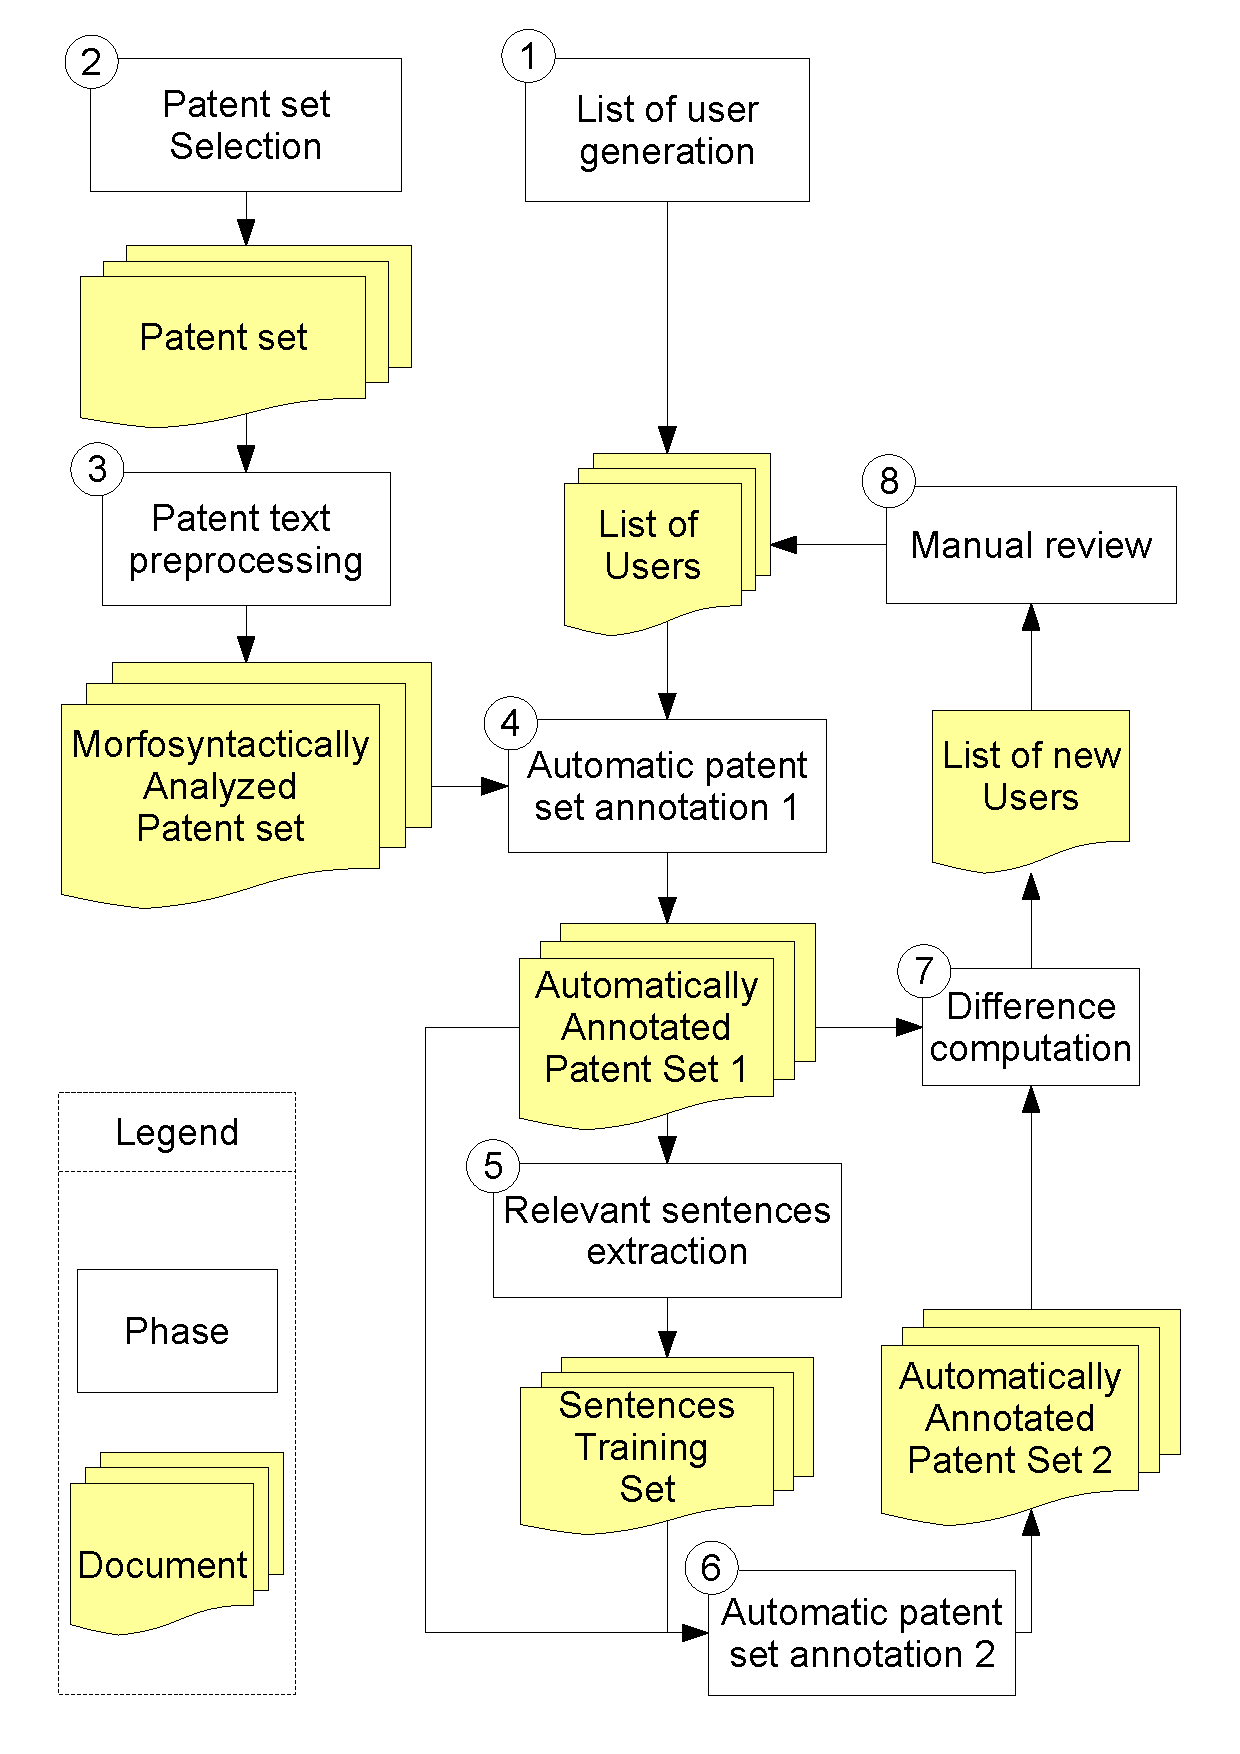
\includegraphics[width=0.8\linewidth]{_bookdown_files/figures/Process} 

}

\caption{Process flow diagram of the proposed automatic user extraction system from patents. The diagram contains the representation of the documents and the operations performed on them. The process takes in input a patent set and a list of users and produces a list of new users as output.}\label{fig:procesuser}
\end{figure}

\subsubsection{List of users generation}\label{sourc}

To generate the input list of users, we used two different approaches: a
bottom-up approach and a top-down approach. The bottom-up approach is
based on the merge of lists from heterogeneous sources. In the present
work we used the following lists of entities:

\begin{itemize}
\item
  \emph{Lists of jobs} :\citep{listjobs}, 11.142 entities
\item
  \emph{Lists of sports and hobbies}:
  \citep[\citet{listhob2}]{listhob1}, 9.660 entities;
\end{itemize}

\emph{List of animals}: \citep{listan}, 600 entities;

\begin{itemize}
\item
  \emph{Lists of patients}: \citep[\citet{listpat2}]{listpat1},14.609
  users;
\item
  \emph{List of generic words}: manually generated. It contains users
  with a higher level of abstraction (such as \emph{person} or
  \emph{human being}), 56 items.
\end{itemize}

Bottom-up approach produced a list of 35.767 entries.

Afterwards, a top-down approach was applied. Starting from the list
generated with the bottom-up approach, we looked for alternative methods
to indicate a user, finding defined word patterns. The most relevant
are:

\begin{itemize}
\tightlist
\item
  Patterns like ``hobby\_term + practitioner'' for the hobbies;
\item
  Patterns like ``person who has + disease\_term'' or ``suffering from +
  disease\_term'' for the diseases;
\item
  Patterns like ``practitioner of + sport\_term'' for sports.
\end{itemize}

Top-down approach generated a total of 41.090 entries.

The whole process generated a total of 76.857 users and gave us a
reasonable number of terms to be used in the next step of the process.

Obviously our lists have a limited coverage and, therefore, they do not
contain all variations of a certain user. For instance, the lists miss
some users belonging to the classes mentioned above (e.g.~new jobs
emerged in the last years) and all the alternative ways for referring to
a user we do not spotted in the top-down approach. For example our lists
miss jobs like \emph{data analyst}, \emph{lap dancer},
\emph{undertaker}, \emph{mortician} and \emph{thief} or patients with
emerging diseases like \emph{work-alcoholic} and \emph{web-addicted}. In
addition, our lists miss a class of users related to religious groups,
containing users like \emph{christians} or \emph{jewish}. Such terms
have intentionally \textbf{not} been introduced in the input list
because we considered these terms as candidates to be extracted by the
process in our case study .

\subsubsection{Patent set selection}\label{patsel}

Our choice of patent sets aimed at challenging our system to find new
users missing in the input list. To reproduce a patent set selection, we
took into consideration the International Patent Classification (IPC)
\citep{wipo1}. IPC is a hierarchical system of patent classes
representing different areas of technology. Then, we wondered which
classes could contain new users according to our seed list. Furthermore,
IPC class A, which is the first level in IPC differentiation, is based
on human necessities. For this reason, we assumed that in this class we
would have found likely users from patents texts.

\subsubsection{Patent text analysis}\label{patent-text-analysis}

Our Entity Extraction system is composed by a set of sequential phases.
The first three phases are related to the linguistic annotation:
sentence splitting and tokenization, part of speech tagging and
lemmatization. Then, the patent set is analyzed by the entity extractor,
specialized for users extraction. A more detailed description of each
phase is:

\begin{itemize}
\item
  Sentence splitting and Tokenization: These processes split the text
  into sentences and then segment each sentence in orthographic units
  called tokens. In our system, sentence splitting plays a key role
  since thanks to a given word, it is possible to find sentences where
  the word is used. Finding correct boundaries for a specific word
  allows to dramatically reduce the space to retrieve its surrounding
  contexts.
\item
  POS tagging and Lemmatization: The Part-Of-Speech tagging (or POS
  tagging) is the process of assigning unambiguous grammatical
  categories to words in context. It plays a key role in NLP and in many
  language technology systems. For the present application we used the
  most recent version of the Felice-POS-tagger described in
  \citep{dell2009ensemble}. Once the computation of the POS-tagged text
  is completed, the text is lemmatized according to the result of this
  analysis.
\item
  Semi-automatic Users Annotation: The Users Extraction tool is based on
  supervised methods. Such methods require an entity annotated corpus in
  order to extract new entities from unseen documents. A semi-automatic
  method has been used to generate an annotated corpus of users to avoid
  manual annotation of a patent set. The method is a projection of the
  list of users on the patent set defined in section @ref\{patsel\}. The
  list of users described in section @ref\{sourc\} is cleaned to avoid
  linguistic ambiguities when projecting these entities on the corpus.
  For example, the term \emph{``guide''} has two different meanings when
  used as a verb or as a noun. Furthermore, as a noun it could indicate
  a component of a system (guide for mechanical parts) or a person
  (someone employed to conduct others) and therefore a user. Avoiding
  ambiguities is a crucial aspect to produce an informative training
  set, so ambiguous words were pruned.
\end{itemize}

The entity annotation schema for a single token is defined using a
widely accepted BIO annotation scheme \cite{ramshaw}:

\begin{itemize}
\tightlist
\item
  \textbf{B-USE}: the token is the beginning of an entity representing
  an User;
\item
  \textbf{I-USE}: the token is the continuation of a sequence of tokens
  representing an User;
\item
  \textbf{O}: for all the other cases.
\end{itemize}

\subsubsection{User Entity Extraction}\label{user-entity-extraction}

The Users extraction problem is tackled by the implementation of a
supervised classifier that is trained on an annotated patent set. Thus,
the patent set is linguistically-annotated, using the steps described
above and entity-annotated, exploiting the semiautomatic annotation
process executed in the previous steps.

Given a set of features the classifier trains a statistical model using
the feature statistics extracted from the corpus. For each new document
the trained model assigns to each word the probability of belonging to
one of the classes previously defined (B-USE, I-USE, O).

In our experiments the classifier has been trained using two different
learning algorithms: Support Vector Machines (SVM) using the LIBSVM
library \citep{libsvm} configured to use a linear kernel and Multi Layer
Perceptron (MLP) implemented using the Keras library \citep{libkeras}.
It has been proven that LSTM methods are well suited for similar NER
task. Anyway, we chose SVM and MLP method to study how two wheel
established state of the art classifiers perform on the specific task of
user extraction from patents and to evaluate their performance in terms
of precision and computational effort. We also think that the popularity
of these methods increment the reproducibility of the work.

The classifier uses different kind of features extracted from the text:

\begin{itemize}
\item
  \emph{linguistic features}, i.e.~lemma, Part-Of-Speech, prefix and
  suffix of the analyzed token;
\item
  \emph{contextual features}, the linguistic characteristics of the
  context words of the analyzed token; in addition the entity category
  of the previous token is considered;
\item
  \emph{compositional features}, combinations of contextual features and
  linguistic features. i.e.~Part-Of-Speech of the previous word and the
  lemma of the current word. These extra features allow to infer
  statistics on the interaction of the combined features that can not be
  captured by a linear SVM model.
\item
  \emph{word2vec features}: vector representations of words computed by
  the \emph{word2vec} \citep{word2vec1} tool.
\end{itemize}

\emph{Word2vec} is a NLP tool able to produce word representations
exploiting big corpora. The main property of the vectors produced by
\emph{word2vec} is that words sharing similar contexts have similar
vector representations. By using word vectors instead of the
corresponding words we were able overcome the problem of the limited
lexical knowledge in the training phase. Using these features and
excluding all the others (delexicalized model) we expected that the
resulting user extraction system had a lower precision and an higher
recall in the classification phase. We presumed to find new users not
contained in the input seed list.

\subsubsection{Manual Review of the new list of users}\label{manrev}

It is still possible that the classification process creates false
positive results (words labeled as users that do not match the
definition in section @ref\{theuse\}). Thus, it is necessary to make a
manual review of the extracted entities with the aim of evaluating the
output.

\subsubsection{Results}\label{results}

The following section describes the performances of the automatic users
extraction process on two different patent sets. To test the system four
experiments were conducted\}. Finally the performances and the outcomes
of the system are shown and discussed.

Following the guidelines for the patent set selection described in
section \ref{patsel}, we examined two patent sets belonging to the IPC
class A:

\begin{itemize}
\tightlist
\item
  \textbf{A47G33}. The IPC definition of the subclass is
  \emph{``religious or ritual equipment in dwelling or for general''}.
\item
  \textbf{A61G1-A61G13}. The IPC definition of the subclass A61G1 is
  \emph{``Stretchers''} while the definition of the subclass A61G13 is
  \emph{``Operating tables; Auxiliary appliances therefor''}.
\end{itemize}

We extracted from the private Errequadro s.r.l. \citep{errequadro}
database a random sample of 2.000 patents from each IPC class. For each
patent set we applied the semiautomatic set annotation process by
projecting the input list of users on the morphosyntactically analyzed
patent set. After this process, each semi-automatically annotated patent
set was split in two parts: the first was used as training set for the
user extractor, and the second one was used as test set.

To build an informative training set, from the semi-automatically patent
set we selected a subset of sentences containing at least one user. The
size of the training set in both cases is approximately composed by
600.000 tokens. For each patent set table \ref{tab:patent set-details}
shows the number of sentences of the training set, the number of
sentences of the test set, and the number of distinct users in the
training set (re-projected by the semi-automatic annotation process).

ref ---\textgreater{} patent set-details

\begin{table*}[!h] %[td!]
  \scriptsize
        \centering
        \begin{tabular}{cccc}
                        \toprule
        \textit{patent set group } &  \textit{\#Sentences - training} & \textit{\#Sentences - test}  & \textit{\#Distinct users projected on training} \\
                        \midrule
         A47G33 & 13.364 & 214.029 & 126   \\
       A61G1-A61G13 & 15.108 & 2.520.350 & 121   \\
        \bottomrule[1pt]
        \end{tabular}
        \caption{\small Statistics related to the patent set groups analyzed in the case study}
       % }
        \label{tab:patent set-details}
\end{table*}

We chose two orders of magnitude for the sentences test-set to test the
efficiency of multiple configurations of the system.

To test the performances of the implemented user extractor, we devised
four different configurations. Each configuration uses a specific
learning algorithm and a set of features to build the statistical model.
The main purpose of this procedure is to find the configurations that
better perform in the user extraction task. In addition, the different
behaviour of the system in the classification phase is studied. In
tables \ref{tab:extractor-configurations} and \ref{tab:feat-confs} are
reported the detailed configurations used in our experiments.

\begin{table*}[!h] %[td!]
 \footnotesize
        \centering
        \begin{tabular}{cc}
                        \toprule
        \textit{Feature group} &  \textit{Context Window} \\
                        \midrule
        Lemma unigrams & $[-2, -1, 0, 1]$  \\
        Lemma bigrams & $[(-1 ,0), (0, 1)]$ \\
        Word bigrams &  $[(-1 ,0), (-2, -1), (0, 1), (1, 2)]$ \\
        Word trigrams &  $[(1, 0, 1) (-2, 1, 0)]$ \\
         Pos unigrams & $[-2, -1, 0, 1]$  \\
         Pos bigrams &  $([(-2, -1) (-1, 0), (0,1)])$  \\
       Compositional feature \#1 & $(POS_{-1}, Lemma_{0})$ \\
       Compositional feature \#2 & $(Lemma_{-1}, Lemma_{0})$ \\
         Compositional feature \#3 & $(Lemma_{0}, Lemma_{1}) $ \\
                  Compositional feature \#4 & $(POS_{0}, Lemma_{1}) $ \\
         Compositional feature \#5 & $(NER_{-1}, Lemma_{0}) $ \\
         Word2vec & [-2, -1, 0, 1, 2] \\
        \bottomrule[1pt]
        \end{tabular}
        \caption{\small Context windows of the extracted features considering 0 as the 
        current analyzed token.
        }
        \label{tab:feat-confs}
\end{table*}

By using the first and the second configuration we expected to have a
higher precision in the classification phase, since explicit lexical
information is used in the training phase. For the same reason we
expected to have low recall in classification phase. On the other hand,
the third and fourth configurations are delexicalized: lexical
information is provided by word vectors computed by word2vec\_. In these
two configurations we expected to have an higher recall and a lower
precision, due to the characteristics of the computed vectors explained
before. To limit errors when using the \emph{word2vec} features, some
linguistically motivated filtering rules were introduced. Specifically,
sequences of tokens classified as users were constrained from the
following categories: verbs, adjectives not preceded by articles,
articles and adverbs.

To evaluate the whole user extraction process in each experiment, we
defined some evaluation measures. Each measure was introduced to
evaluate the characteristics of the extraction system concerning the
configuration applied.

These measures are:

\begin{itemize}
\tightlist
\item
  Training time: time needed to create the statistical model using the
  training set;
\item
  Test time: time needed to re-annotate the semi-automatically annotated
  patent set;
\item
  Number of extracted users: number of unique entities classified as
  user in the automatically annotated patent set;
\item
  Number of known users: number of distinct extracted users in the
  automatically annotated patent set and belonging to the list of user
  in input;
\item
  Number of new users: number of distinct entities classified as user in
  the automatically annotated patent set and not belonging to the input
  list of users;
\item
  Number of new correct users: number of distinct entities considered as
  user and as correct after a manual review;
\item
  Precision: ratio between the number of new distinct correct users and
  the total number of new distinct users;
\item
  Gain: ratio between the number of new distinct correct users and the
  number of re-projected distinct users on the training set.
\end{itemize}

\{

\begin{table*}[!h] %[td!]
      \tiny
        \begin{tabular}{lccccccccc}
         \hline
               Experiment  &  Training time & Test Time & Extracted  &  Known &  New  &  New correct &  New wrong & Prec. (\%) & Gain (\%) \\

            \midrule
                        \multicolumn{10}{c}{\textit{A47G33}}\\

                  \midrule
    1 (SVM) & 83m  & 321m & 161 & 93 &  68 & 47 & 21  &  69.11 & 37.30  \\
    2 (MLP) & 1911m  & 9091m & 196 & 55 &  141 & 27 & 114  &  19.15 & 21.42  \\
    3 (MLP-W2V) &  165m & 246m &  162 & 35 &  127 & 45 & 82   & 35.43 & 35.71 \\
    4 (SVM-W2V) &  1265m & 4310m &  121 & 29 &  92 & 45 & 47   & 48.91 &  35.71  \\
     \hline
            \multicolumn{10}{c}{\textit{A61G1-A61G13}}\\
                \midrule

   5 (SVM)  & 148m & 3443m &  302 & 120 &  182 & 88 & 108  & 48.35 & 72.72  \\
   6 (MLP)  & 1818m & --- &  --- & --- &  --- & --- & ---  & --- & ---  \\
    7 (MLP-W2V)   & 333m & 3530m &  305 & 38 &  267 & 44 & 230   & 16.48  & 36.36 \\
    8 (SVM-W2V)  & 1268m & 47020m &  313 & 49 &  264 & 74 & 197   & 28.03 & 61.15 \\


    \bottomrule
        \end{tabular}
            \caption{\small Comparison of the values of the defined metrics across all the experiments.
              The patent set annotation in the experiment (6) was not performed due to the computational costs.
              All the experiments were run on a machine provided with 10 AMD Opteron(tm) 6376 processors.}
               \label{tab:runs-data}

  \end{table*}

\}

Table \ref{tab:runs-data} reports the values of the defined metrics
across all the experiments run on the two patent sets.

For what concerns training and test time of the automatic patent set
annotation, it's clear that the configuration based on the SVM learning
algorithm without the \emph{word2vec} features performs better in both
the experiments (1, 5). When the features based on \emph{word2vec} are
introduced, the configuration based on the MLP learning algorithm is the
fastest both in training and test time (3, 6): it is due to the fact
that keras implementation of this algorithm exploits all the available
CPU cores of the system. On the other side, the MLP algorithm does not
scale properly with a higher number of features, as seen in training and
annotation time in the experiment (2). In addition, we could not perform
the patent set annotation in the experiment (6), since it would have
required more than 60 machine days to complete the process. When
\emph{word2vec} features are introduced, the patent set annotation based
on the SVM algorithm is 10 times slower than the MLP algorithm.

For what concerns the precision in the automatic patent set annotation,
the SVM configuration without \emph{word2vec} features is clearly the
more reliable: the precision values are from 1.5 to 2 times higher in
the experiments (1, 5) in contrast to the other experiments. The higher
precision is justified by the fact that the configurations based on
\emph{word2vec} features lack explicit lexical information: words with
very similar contexts are represented by similar \emph{word2vec}
vectors, probably leading to errors in the classification phase. On the
other hand, the use of \emph{word2vec} vectors aims at extracting
entities that would not be extracted by considering explicit lexical
information only.

Finally, for what concerns information gain, the same amount of new
information (21-37\%) is extracted in the experiments on the A47G33
patent set. The gain values drastically change in the experiments on the
A61G1-A61G13 patent set: in the experiments (5, 8) a gain between 61\%
and 72\% is obtained: it is due to the size of this patent set in
comparison to the A47G33 one. In the experiment (7), despite the
introduction of \emph{word2vec} features, a gain of 36\% is obtained.
This fact, in conjunction with the non-feasibility of the experimental
configuration 6, shows how MLP systems lack in efficacy and efficiency
(in entity extraction in patent domain) when the test-set has an order
of magnitude of millions of sentences. We think that this result is
relevant, based on our experience with practical applications.

Furthremore, a way to maximize the overall informative gain is to merge
the results of all manually reviewed user extractions obtained by
executing the patent set annotation process with all possible
configurations.

The overall informative gain of the merging process is related to
intersections that occur among the results obtained by the patent set
annotation process in each configuration: the less the intersections,
the more the overall informative gain obtained. In table
\ref{tab:merge-data} is shown the overall gain obtained by merging
results of the manually reviewed extractions in each patent set.

\{

\begin{table*}[!h] %[td!]
    \footnotesize
    \centering
    \begin{tabular}{ccc}
      \hline
      Configuration & A47G33 - Gain (\%) & A61G1+A61G11 - Gain (\%) \\
      \midrule
          SVM & 37.30 & 72.72 \\
          MLP & 21.42 & --- \\
          MLP-W2V & 35.71 & 36.36 \\
          SVM-W2V & 35.71 & 61.15 \\
          SVM $\cup$ MLP & 52.38 & --- \\
          SVM $\cup$ MLP-W2V & 69.84 & 126.44 \\
          SVM $\cup$ SVM-W2V & 73.01 & 103.30 \\
          MLP $\cup$ MLP-W2V & 55.55 & --- \\
          MLP $\cup$ SVM-W2V & 57.14 & --- \\
          MLP-W2V $\cup$ SVM-W2V & 59.52 & 76.30 \\
          SVM $\cup$ SVM-W2V $\cup$ MLP-W2V & 90.47 & 140.49 \\
          SVM $\cup$ MLP $\cup$ MLP-W2V & 82.53 & --- \\
          SVM $\cup$ MLP $\cup$ SVM-W2V & 85.71 & --- \\
          MLP $\cup$ SVM-W2V $\cup$ MLP-W2V & 77.77 & --- \\
          SVM $\cup$ MLP $\cup$ SVM-W2V $\cup$ MLP-W2V & 103.17 & --- \\
          \bottomrule
        \end{tabular}
    \caption{\small Gain obtained by merging correct entities extracted from each patent set annotation.}
    \label{tab:merge-data}

  \end{table*}

\}

The table shows that the merging process of manually reviewed entities
extracted from each patent set annotation run effectively contributes to
increase the overall informative gain. For instance in the A47G33 patent
set an overall gain of 103.17\% is obtained, tripling the best result
achieved by the extraction performed using the best single
configuration. Good results are also achieved in the A47G33 patent set
user extraction. In this case an overall gain of 140.49\% is obtained,
doubling the best result achieved by the extraction performed using the
best single configuration.

The results shown in section 5 prove that if the goal of the extraction
is to reach the maximal recall, an ensemble method (combining the output
of multiple classifier) over-performs every single classifier method.
Anyway, the ensemble approach has clear efficiency issues, because the
time of analysis will be the sum of every single approach time (in
hypotheses of non-parallelization). This leads to a trade off between
the speed of the system and the quality of the results, and whoever
would use the presented system can decide to gain benefit in one or in
another direction.

Finally, tables \ref{tab:result-extraction-dl-a47g33} and
\ref{tab:result-extraction-dlw2v-a47g33} show an overview of extracted
users randomly chosen from the A47G33 patent set (the only one in which
were able to perform all experiments). Each table is divided in two
blocks, representing the results of the extraction performed using a
specific configuration. For each extracted user is shown the
corresponding lemma (the root form), the frequency (how many times that
user appears in the whole corpus) and the total number of patents
containing the user. Users not contained in the starting user list, are
highlighted in bold.

The table shows that the system was able to extract characteristic users
of the patent set. The results are in fact not unexpected for the IPC
class under analysis: this is an evidence of the correct performances of
the proposed system. In other words, the results presented in the table
show that it is possible to train a NER systems able to extract sparse
and valuable information. Such users are the ones that an expert would
manually extract but the NER system does it with an enormous saving in
terms of time and efforts.

Other remarkable results are:

\begin{itemize}
\item
  many newly extracted entities have very low frequency in the patent
  set: it shows that the developed system is able to extract rare
  entities.
\item
  table \ref{tab:result-extraction-dlw2v-a47g33} shows that
  configurations using \textit{word2vec} features are able to find new
  users with a higher frequency in the patent set: it was an expected
  result, since the \textit{word2vec} configurations are not explicitly
  lexicalized and more able to generalize during extraction phase.
\item
  The system is able to extract single words and multi-words.
\item
  Taking into consideration the definition we have given in section
  \ref{theuse}, the system extracts unusual and sometimes borderline
  users. Examples like \emph{saint}, \emph{angel}, \emph{god} and
  \emph{ghost} need discussion that is far beyond the purposes of the
  present paper. These results are a remarkable evidence of the
  human-like generalization ability of the described method.
\end{itemize}

\begin{table*}[!h] %[td!]
    \footnotesize
    \centering
    \begin{tabular}{cccccc}
          \hline
      \multicolumn{3}{c}{SVM} &  \multicolumn{3}{c}{MLP} \\
    \hline
    Lemma & Frequency & \# Patents & Lemma & Frequency & \# Patents  \\
    \hline
female & 801 & 109 & child & 402 & 102  \\
child & 426 & 108 & cleregy member & 128 & 5 \\
guy & 156 & 17 & patient & 113 & 11 \\
patient & 115 & 11 & man & 50 & 26  \\
parent & 70 & 31 & young & 48 & 32 \\
man & 51 & 26 & \textbf{angel} & 29 & 23  \\
merchant & 50 & 6 & dog & 20 & 7  \\
soon & 46 & 29 & artisan & 12 & 12 \\
engineer & 45 & 45 & \textbf{male/female} & 12 & 4  \\
adult & 39 & 23 & hockey player & 7 & 1  \\
young & 35 & 24 &  \textbf{professional}  & 7 & 7   \\
society & 32 & 21 & tennis player  & 7 & 4  \\
\textbf{angel} & 29 & 23 & football player   & 6 & 3 \\
fund raiser & 27 & 4 &  \textbf{ghost} & 5 & 3   \\
priest & 22 & 4 & children  & 5 & 5 \\
cheerleader & 15 & 4 & manager  & 5 & 5  \\
\textbf{fund-raiser} & 11 & 4 & \textbf{spider} & 5 & 5 \\
\textbf{athlete} & 10 & 9 &  \textbf{vandal}  & 5 & 1  \\
\textbf{ghost} & 5 & 5 & \textbf{athlete}  & 4 & 3  \\
\textbf{adulterant} & 3 & 3 & mother  & 4 & 2  \\
\textbf{jew} & 3 & 3 & soccer player  & 4 & 3  \\
\textbf{maid} & 3 & 1 & squirrel  & 3 & 2 \\
\textbf{tourist} & 3 & 3 & \textbf{maid}  & 3 & 1 \\
\textbf{indian} & 2 & 2 & \textbf{god}  & 3 & 2  \\
\textbf{beginner} & 1 & 1 & \textbf{mariner}  & 3 & 3  \\
\textbf{christians} & 1 & 1 &  \textbf{male-female}  & 2 & 2  \\
\textbf{datum entry operator} & 1 & 1 & \textbf{manufacturer}  & 2 & 2  \\
\textbf{expert} & 1 & 1 & \textbf{jew}  & 1 & 1  \\
\textbf{jewish} & 1 & 1 & \textbf{merchandizers} & 1 & 1  \\
\textbf{marinaro} & 1 & 1 & \textbf{parishioner} & 1 & 1 \\
          \bottomrule
        \end{tabular}
            \caption{\small Extracted users from the A47G33 patent set using the SVM and DL configurations.
            New users extracted by the system are reported in bold.
            }
              \label{tab:result-extraction-dl-a47g33}
  \end{table*}

\begin{table*}[!h] %[td!]
    \footnotesize
    \centering
    \begin{tabular}{cccccc}
          \hline
      \multicolumn{3}{c}{SVM-W2V} & \multicolumn{3}{c}{MLP-W2V}   \\
    \hline Lemma & Frequency & \# Patents & Lemma & Frequency & \# Patents \\
    \hline
  child & 152 & 68 & clergy member & 124 & 5 \\
 clergy member & 124 & 5  & \textbf{crowd} & 36 & 3 \\
  man & 50 & 26 & basketball player & 20 & 5\\
 engineer & 45 & 45 & \textbf{him} & 17 & 8  \\
young & 29 & 24 & woman & 16 & 8   \\
\textbf{choir} & 17 & 1 & \textbf{saint} & 14 & 2  \\ 
 \textbf{infirm} & 13 & 8 & \textbf{youth} & 14 & 2  \\
\textbf{bride} & 9 & 4 &\textbf{angel} & 8 & 4  \\
\textbf{volunteer} & 8 & 6 &\textbf{choir} & 8 & 1   \\
 musician & 6 & 6 & musician & 6 & 6   \\
 boy & 3 & 1 & \textbf{god} & 5 & 1  \\
 children & 3 & 3 & children & 3 & 3   \\
 girl & 3 & 2 & guy & 3 & 3  \\
 \textbf{creature} & 2 & 1 & infant & 3 & 3  \\
\textbf{deceased} & 2 & 1 & priest & 3 & 3  \\
\textbf{jewish} & 2 & 2  & \textbf{bride} & 2 & 2  \\
\textbf{person} & 2 & 2 & \textbf{consumer} & 2 & 2  \\
mother & 2 & 2 & \textbf{everyone} & 2 & 2  \\
 \textbf{audience} & 1 & 1 & \textbf{him/her} & 2 & 2  \\
\textbf{boyfriend} & 1 & 1 & \textbf{spectator} & 2 & 2   \\
\textbf{derby member} & 1 & 1 & farmer & 2 & 1   \\
\textbf{gift giver} & 1 & 1 & youngster & 2 & 2  \\
 \textbf{handicapped} & 1 & 1 & \textbf{boyfriend} & 1 & 1  \\
\textbf{jesus} & 1 & 1 & \textbf{grandparent} & 1 & 1  \\
 \textbf{saint} & 1 & 1  & \textbf{subject} & 1 & 1 \\
husband & 1 & 1  & clown & 1 & 1 \\
lady & 1 & 1  & husband & 1 & 1 \\
runner & 1 & 1 & runner & 1 & 1  \\
 society & 1 & 1 & society & 1 & 1  \\
teenager & 1 & 1 & tennis player & 1 & 1  \\
          \bottomrule
        \end{tabular}
            \caption{\small  Extracted users from the A47G33 patent set using the SVM-W2V  and MLP-W2V configurations.
            New users extracted by the system are reported in bold.}
              \label{tab:result-extraction-dlw2v-a47g33}

  \end{table*}

The total number of users is 109. 28,2\% (564 on 2.000) of patents in
analysis contains at least one user. This result is an evidence of the
fact that patents actually contain users information, and, considering
the approach we followed, this percentage is an accurate lower
approximation of the actual percentage of patents containing at least
one user.

In figure \ref{patents_per_user} for each user on the x axes is shown
the number of patents in which the user is contained. The distribution
is skewed, with some occurrences showing large numbers and many others
with just one or few occurrences. It is clear that there is a Pareto
like distribution, with the first 20\% of users covering 70\% of total
users in terms of occurrence. It means that some users are more likely
to be cited in patents and many more users that rarely appear. Following
this observations, we can divide users in three groups:

\begin{itemize}
\item
  \emph{Group A}: users that appear in more than 100 patents (5\% of the
  patent set). In our case these are \emph{male}, \emph{child} and
  \emph{female}.
\item
  \emph{Group B}: users that appear in more than 20 patents (1\% of the
  patent set). This group is composed by 13 different users. Some of
  these are \emph{engineer}, \emph{person}, \emph{player}, \emph{adult},
  \emph{angel} and \_guy.
\item
  \emph{Group C}: users that appear in less then 20 patents. This group
  is composed by 93 different users. Some of these are \emph{mother},
  \emph{athlete}, \emph{priest}, \emph{adulterant}, \emph{golfer} and
  \emph{hockey player}.
\end{itemize}

Further research means to study how these users differ from patent set
to patent set. We expect to see similar distribution but with different
content of users. Frequent and non-specific users comprise Group A: in
other patent set we could see differences in terms of entities contained
in this class but its content will stay non-specific. These results seem
to be generic social roles indicating the gender or the age of a person.
Group B is composed of mainly non-specific users and some specific users
that change from patent set to patent set. This class helps to identify
the core users of the patent set. Lastly, Group C contains non-frequent
users that are both specific and non-specific, making it the most
interesting of the three for the purposes of our work. In this group we
find users that are market niches, so the patent that contains these
users is of great interest for marketers and designers. These are both
samples of the more generic users (for example a \emph{mother} is a
\emph{female} and a \emph{hockey player} is a \emph{player}) or specific
users of the patent-set (like \emph{priest}, \emph{fund-raiser},
\emph{doll}, \emph{spouse} and \emph{clergy member}.

\begin{figure}

{\centering 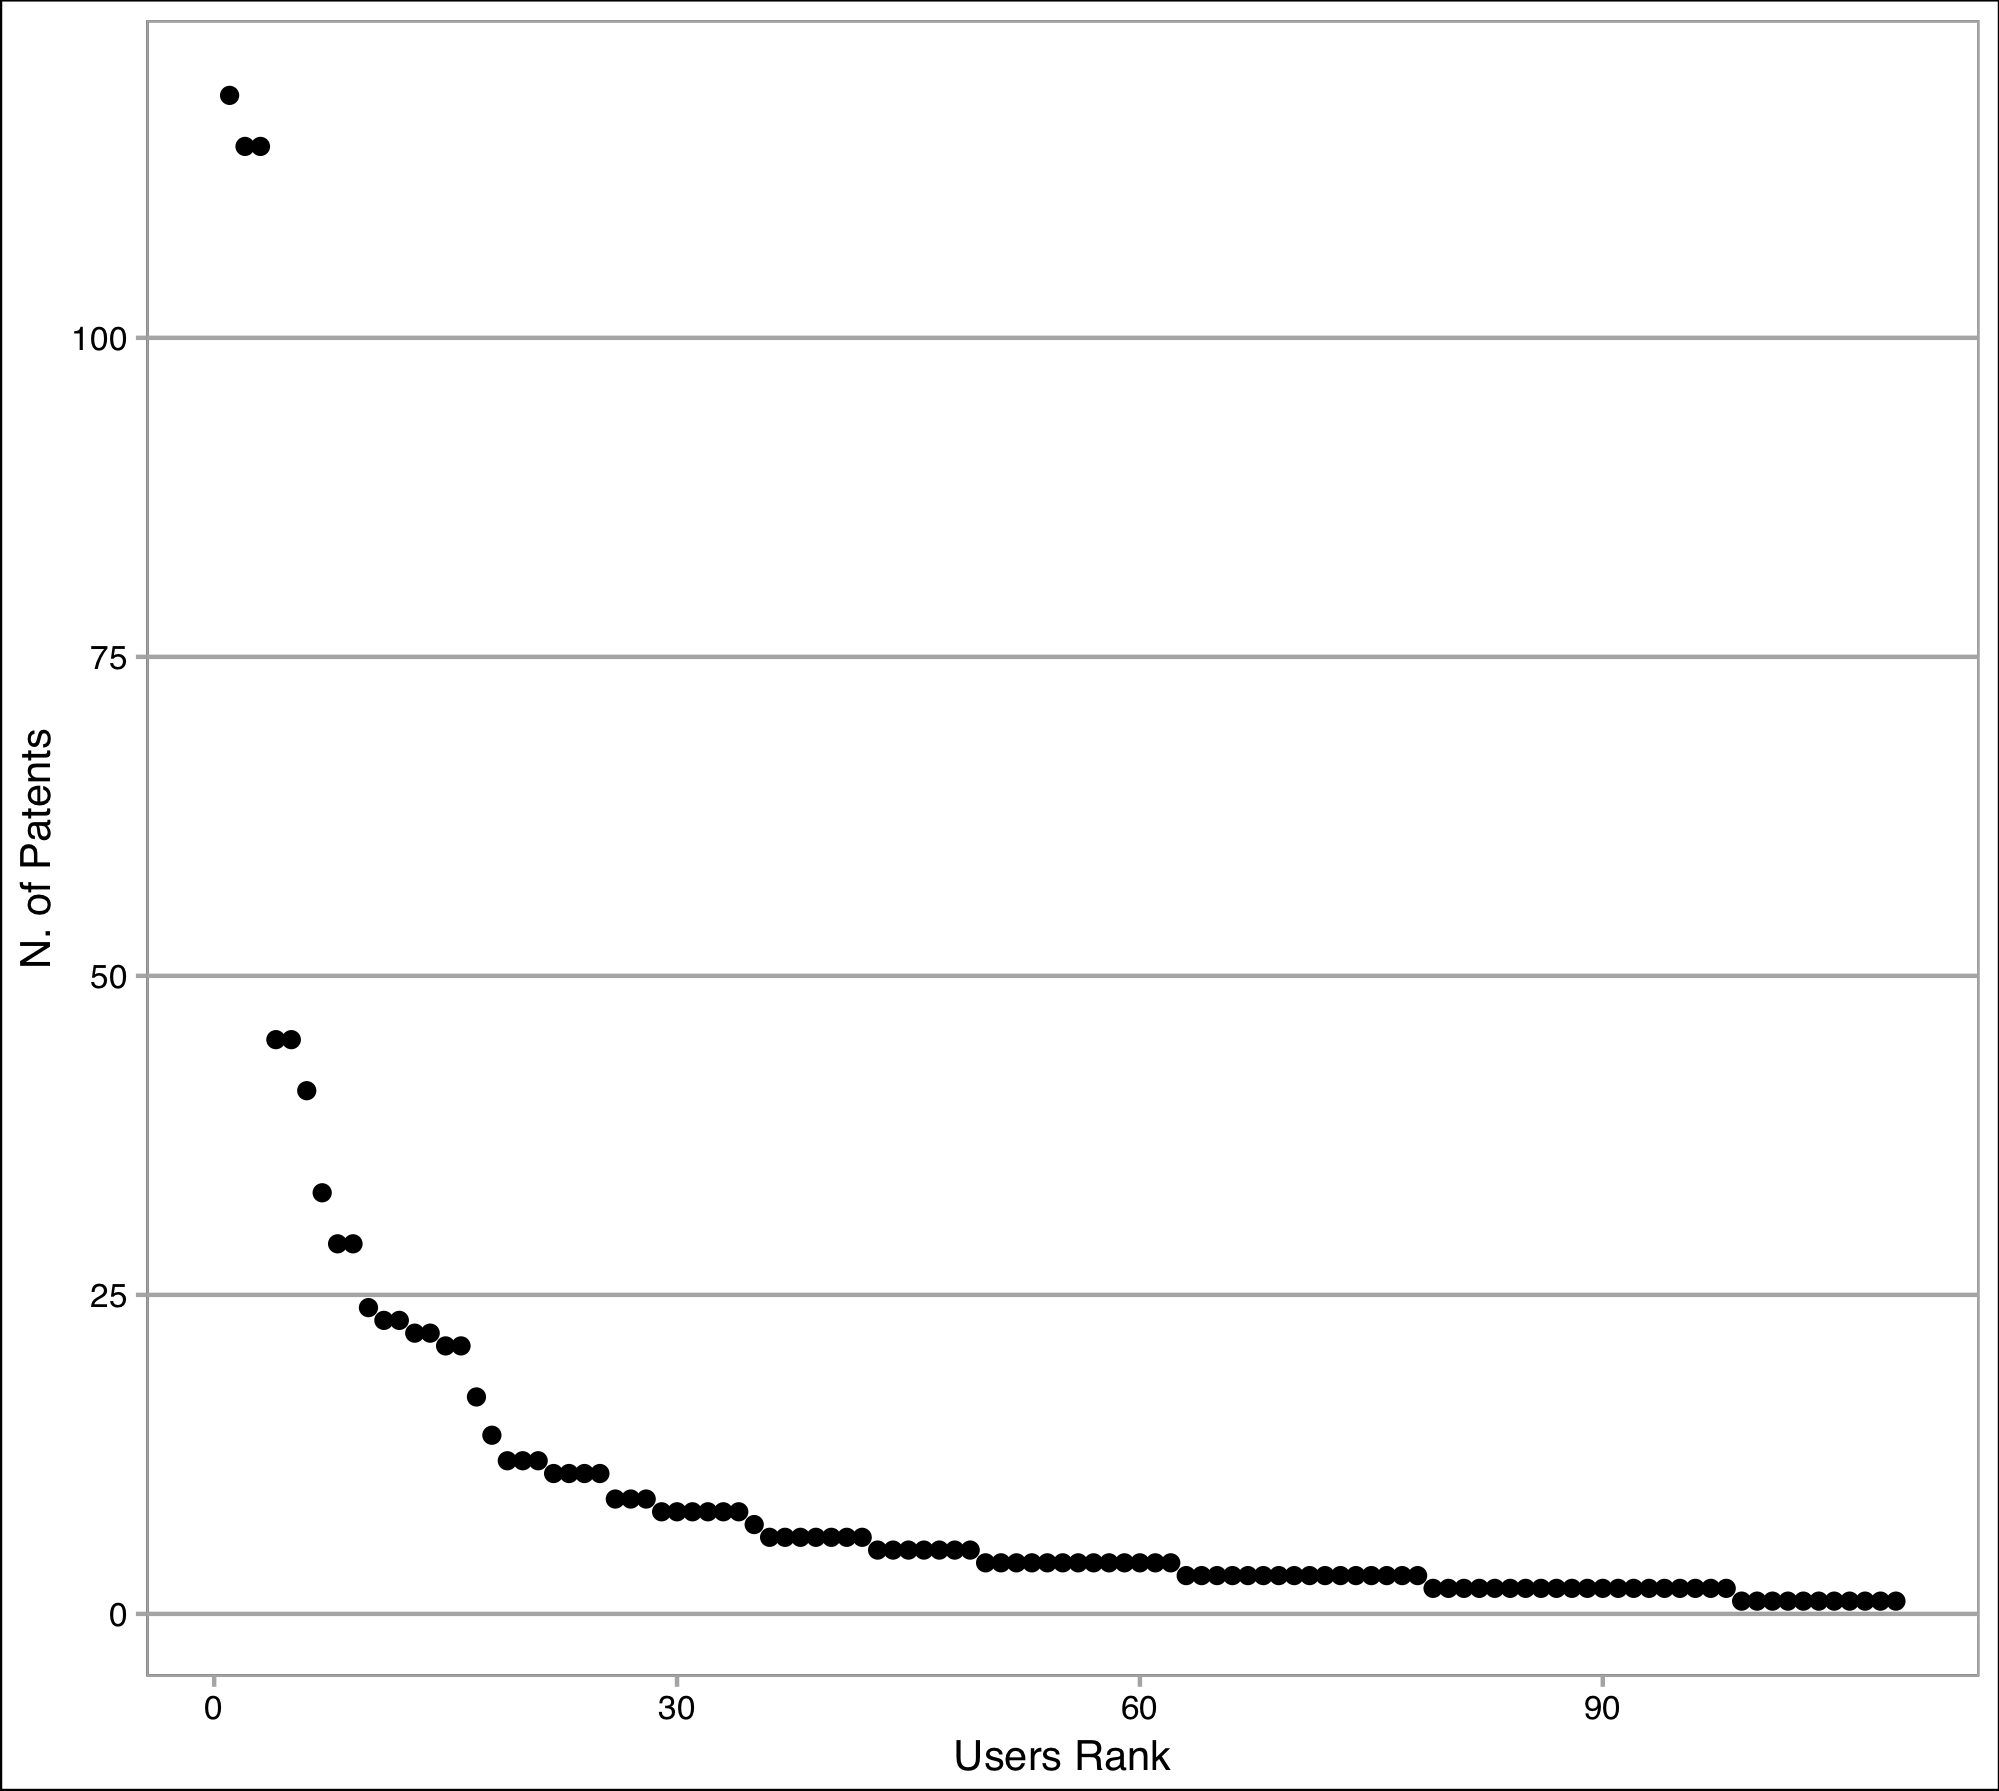
\includegraphics[width=0.8\linewidth]{_bookdown_files/figures/user_rank} 

}

\caption{Process flow diagram of the proposed automatic user extraction system from patents. The diagram contains the representation of the documents and the operations performed on them. The process takes in input a patent set and a list of users and produces a list of new users as output.}\label{fig:userrank}
\end{figure}

\subsection{Advantages and Drawbacks}\label{advantages-and-drawbacks}

\subsection{Trademakrs}\label{trademakrs}

\section{Papers}\label{papers}

\section{Projects}\label{projects}

\section{Wikipedia}\label{wikipedia}

\section{Twitter}\label{twitter}

\section{Job Profiles}\label{job-profiles}

\chapter{Future Developments}\label{future-developments}

\section{Marketing}\label{marketing-1}

\section{Research and Development}\label{research-and-development}

\section{Design}\label{design}

\section{Human Resources}\label{human-resources}

\chapter{Conclusions}\label{conclusions}

We have finished a nice thesis

\chapter{Glossary}\label{glossary}

Morphology= the study of the way words are built up from smaller
meaning-bearing units called morphemes.

\bibliography{papers.bib}


\end{document}
